\RCS$Revision: 342265 $
\RCS$HeadURL: svn+ssh://bainbrid@svn.cern.ch/reps/tdr2/papers/SUS-14-006/trunk/SUS-14-006.tex $
\RCS$Id: SUS-14-006.tex 342265 2016-05-10 19:38:31Z bainbrid $

\newlength\cmsFigWidth
\ifthenelse{\boolean{cms@external}}{\setlength\cmsFigWidth{0.85\columnwidth}}{\setlength\cmsFigWidth{0.4\textwidth}}
\ifthenelse{\boolean{cms@external}}{\providecommand{\cmsLeft}{top}}{\providecommand{\cmsLeft}{left}}
\ifthenelse{\boolean{cms@external}}{\providecommand{\cmsRight}{bottom}}{\providecommand{\cmsRight}{right}}

\cmsNoteHeader{SUS-14-006} 

\title{Additional material for SUS-14-006}

\date{\today}

\abstract{This document contains the auxiliary public material for SUS-14-006.}

\hypersetup{
  pdfauthor={M. Baber, R. Bainbridge, O. Buchmueller, D. Burton,
    M. Citron, A. Elwood, Y. Eshaq, H. Flaecher, A. Garcia-Bellido,
    E. Laird, K. Lo, C. Lucas, J. Marrouche, Z. Meng, T. Sakuma,
    D. Smith, and A. Tapper},
pdftitle={Additional Material for SUS--14--006},
pdfsubject={CMS},
pdfkeywords={CMS, physics, SUSY, jets, missing transverse momentum,
  alphaT} 
}

\maketitle

\clearpage
\begin{figure}[h!]
  \begin{center}
    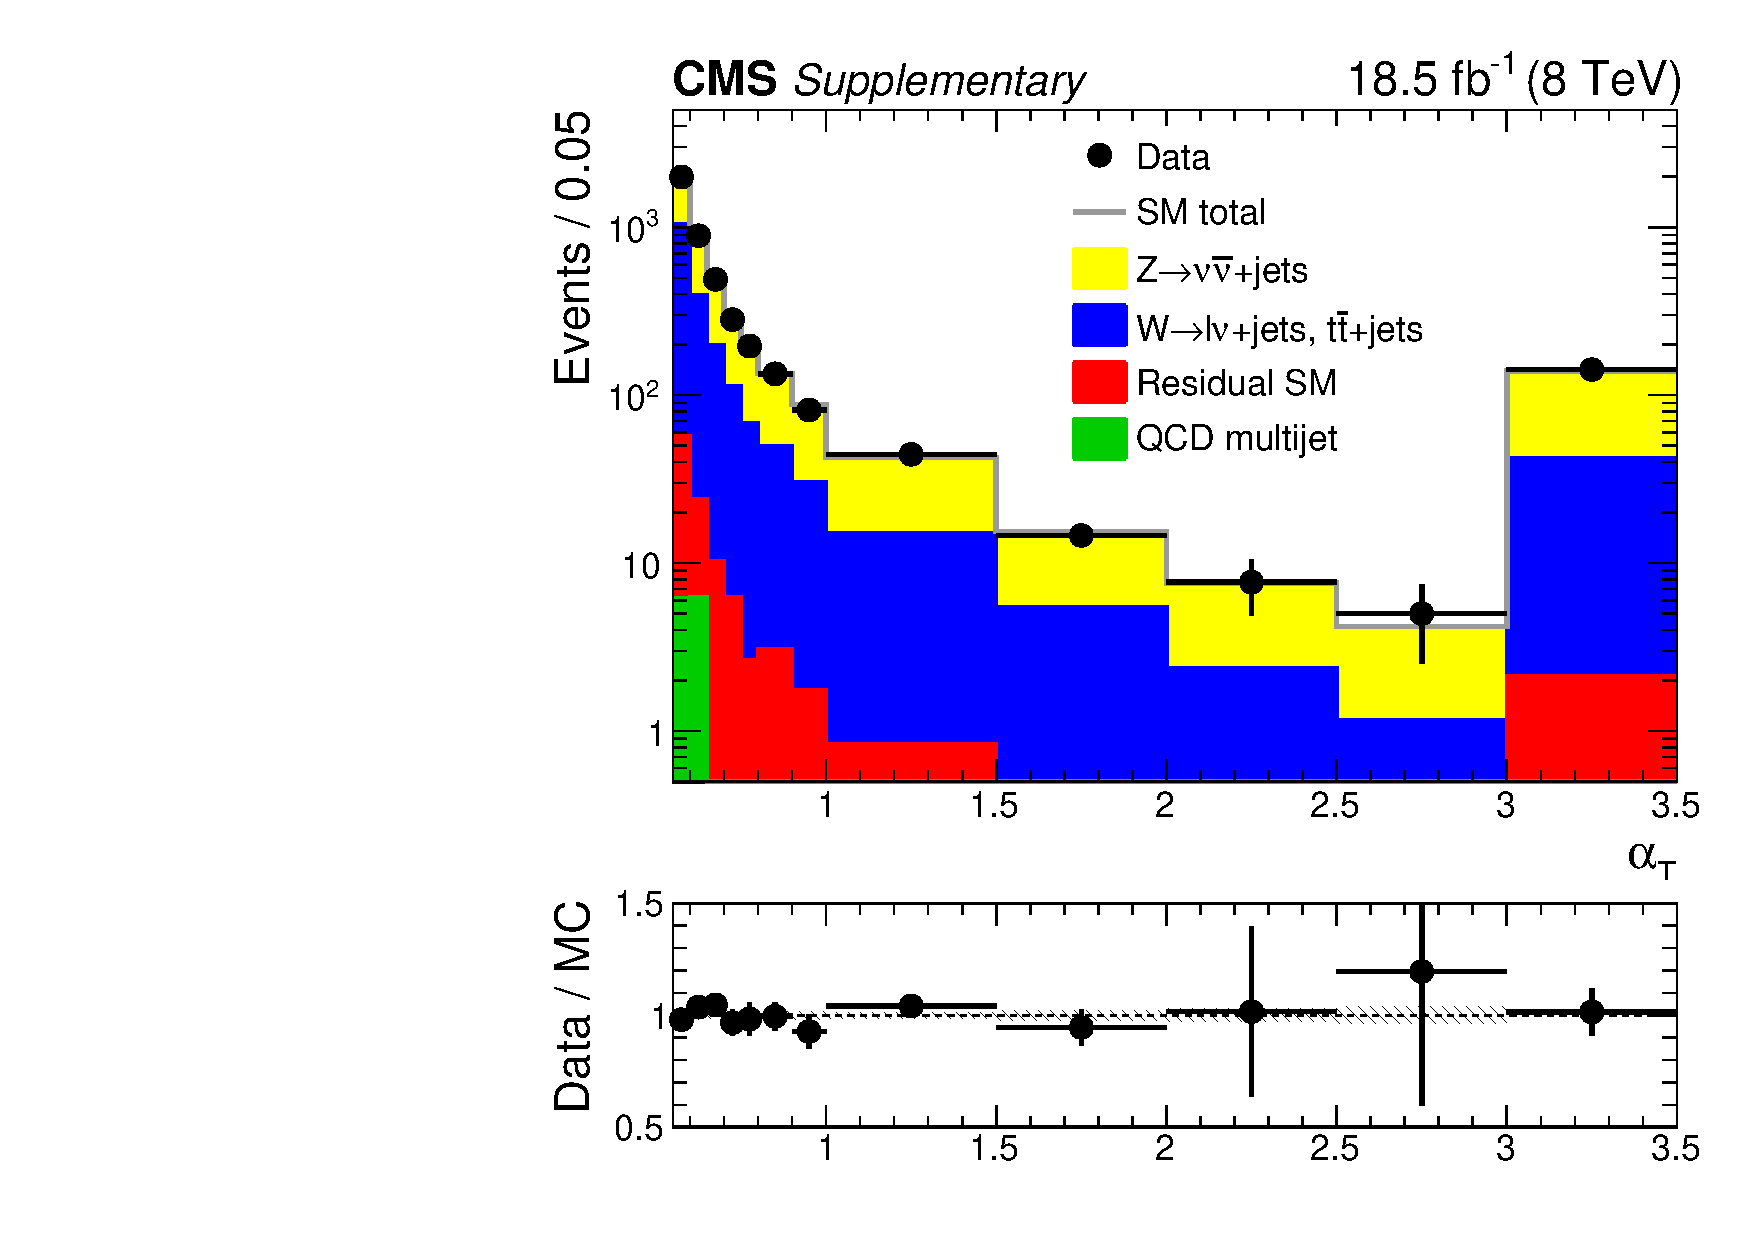
\includegraphics[width=0.7\textwidth]{RootFilesAndTarFiles/AlphaT} \\
    \caption{ (Upper panel) The $\alpha_\text{T}$ distribution
      observed in data for events that satisfy the full signal region
      selection criteria, including the requirements $n_\text{jet}
      \geq 2$, $n_\text{b} \eq 0$, $H_\text{T} > 375\GeV$, and
      $\alpha_\text{T} > 0.55$. Both candidate signal event yields
      observed in data (solid circles) and SM expectations as
      determined from simulation (solid histograms) are
      shown. Contributions from the SM processes of single top quark,
      diboson, Drell-Yan, and t$\text{\bar{t}}$ + gauge boson (W, Z,
      H) production are collectively labelled ``Residual SM''.  The
      statistical uncertainties for the multijet and SM expectations
      are represented by the hatched areas (visible only for
      statistically limited bins). The final bin of each distribution
      contains the overflow events.  (Lower panel) The ratios of the
      binned yields obtained from data and Monte Carlo (MC) simulation
      as a function of $\alpha_\text{T}$. While the search relies only
      on simulation through ratios, these distributions illustrate the
      accuracy of the simulation modelling.  }
  \end{center}
\end{figure}

\clearpage
\begin{figure}[h!]
  \begin{center}
    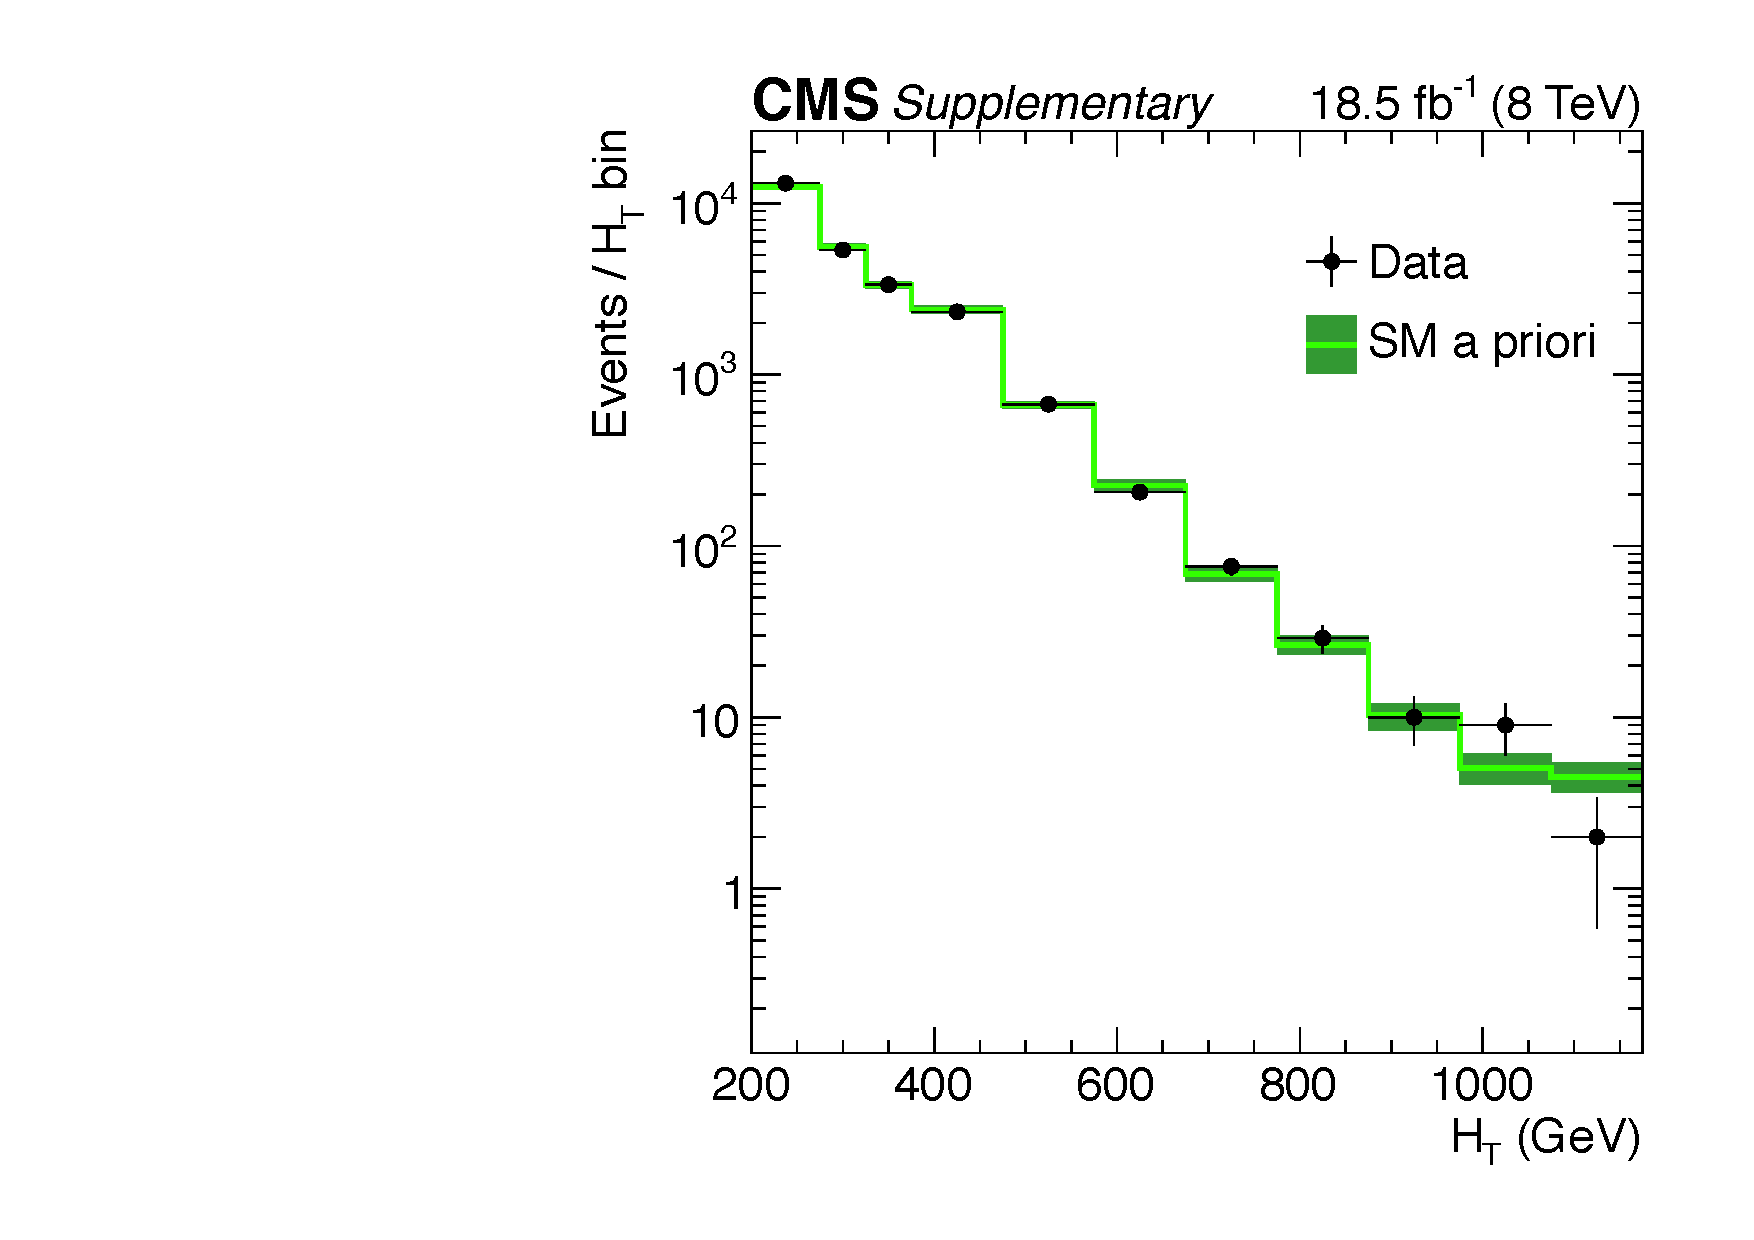
\includegraphics[width=0.7\textwidth]{RootFilesAndTarFiles/eq0b_le3j_prefit_log} 
    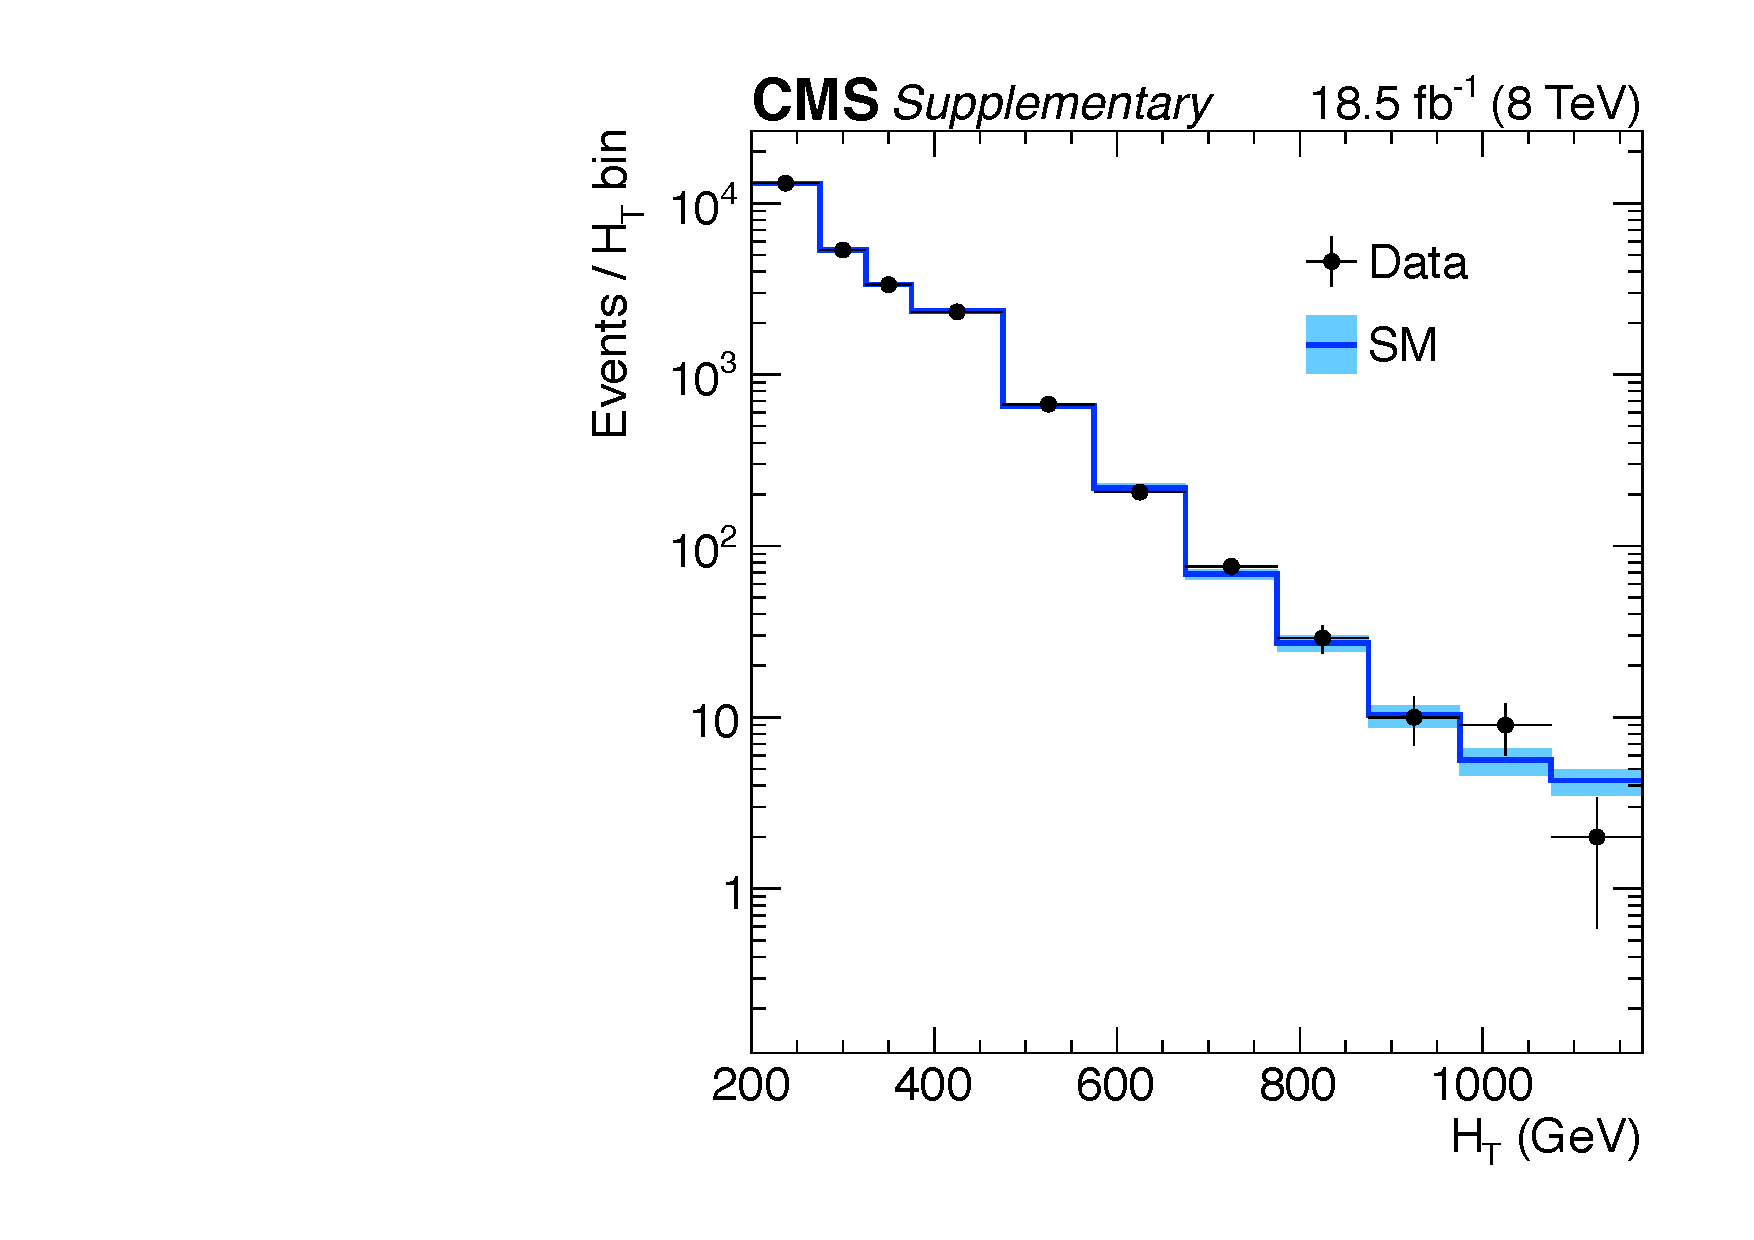
\includegraphics[width=0.7\textwidth]{RootFilesAndTarFiles/eq0b_le3j_postfit_log} \\
    \caption{\label{fig:best-fit-0b} Candidate signal event yields
      observed in data (solid circles) and SM expectations with their
      associated uncertainties (solid lines with bands) in bins of
      $H_\text{T}$ for events that satisfy $2 \geq n_\text{jet} \geq
      3$ and $n_\text{b} = 0$. (a) SM a priori
      expectations. (b) SM expectations from the fit including the
      signal region. }
  \end{center}
\end{figure}

\clearpage
\begin{figure}[h!]
  \begin{center}
    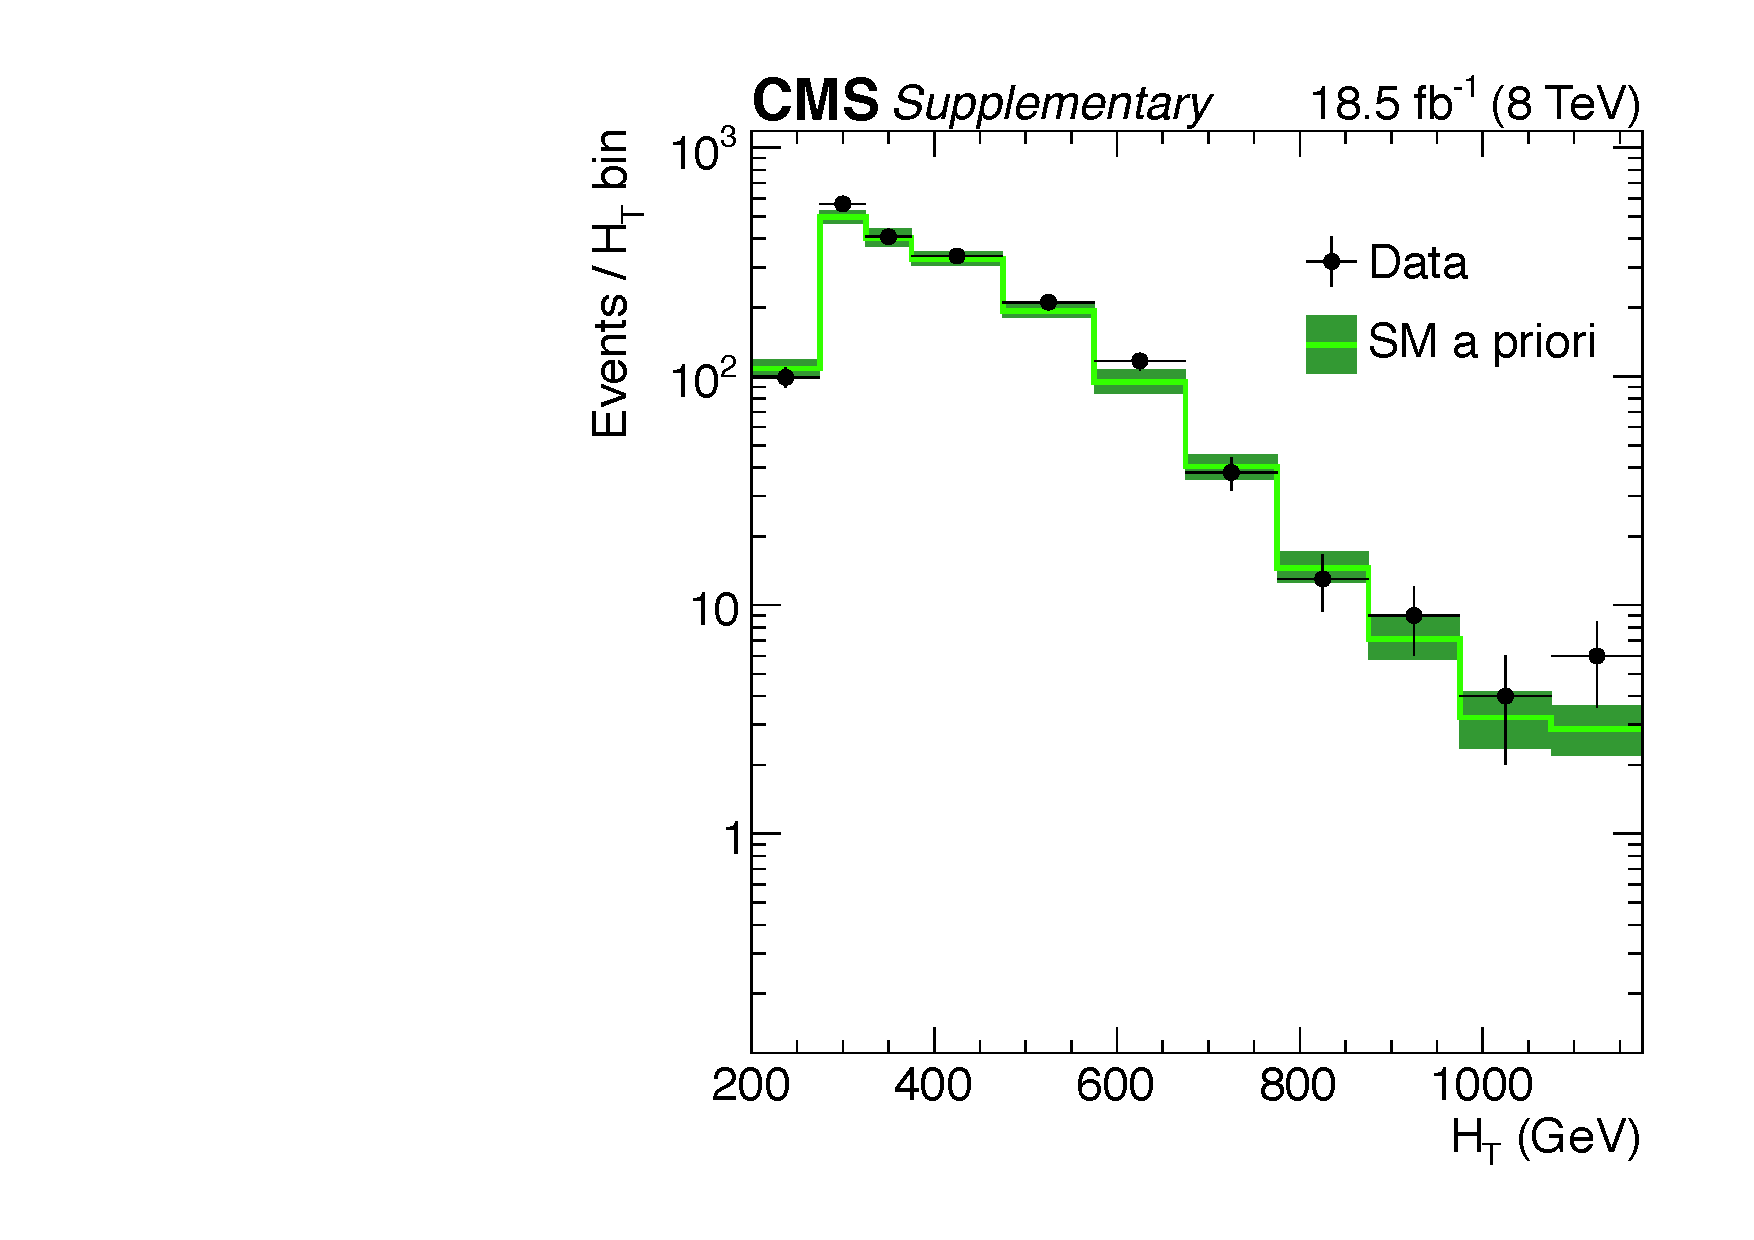
\includegraphics[width=0.7\textwidth]{RootFilesAndTarFiles/eq0b_ge4j_prefit_log} 
    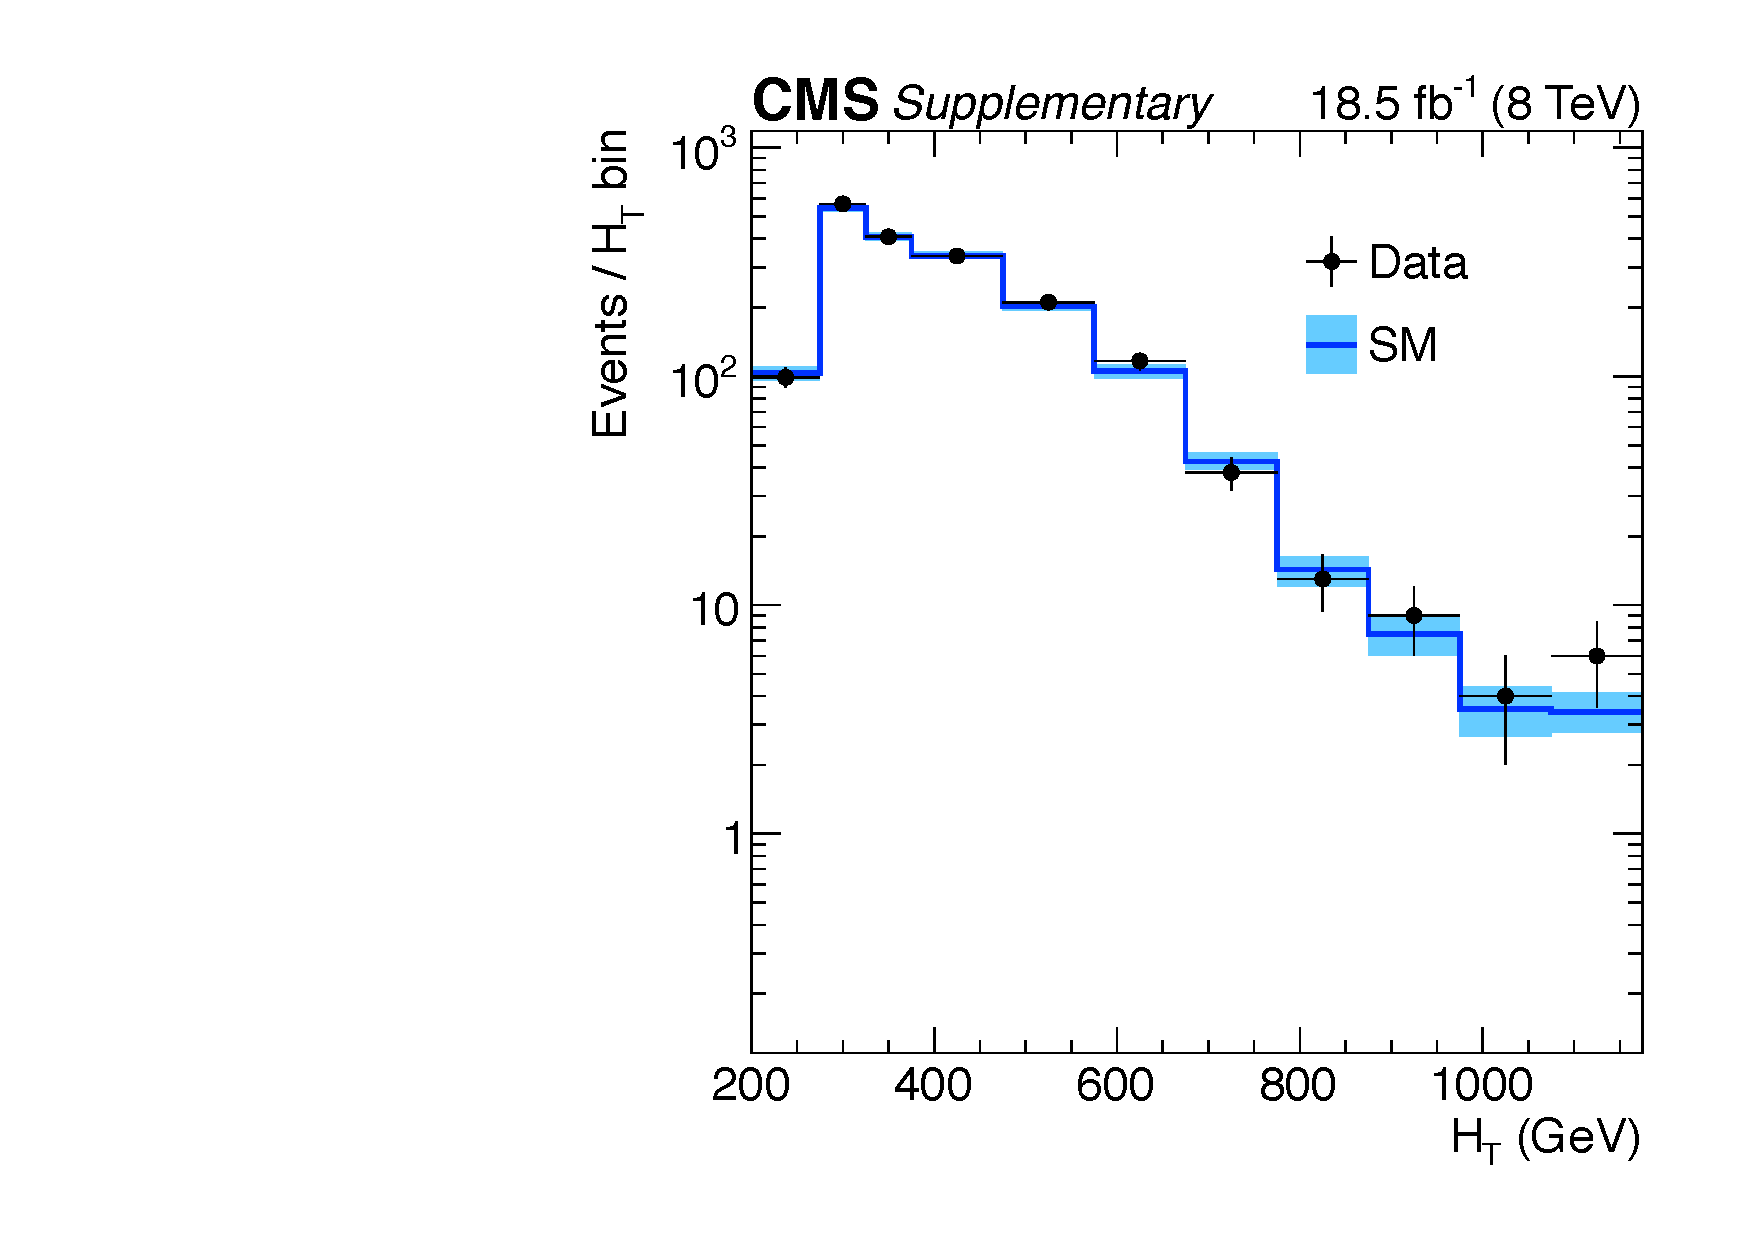
\includegraphics[width=0.7\textwidth]{RootFilesAndTarFiles/eq0b_ge4j_postfit_log} \\
    \caption{\label{fig:best-fit-0b} Candidate signal event yields
      observed in data (solid circles) and SM expectations with their
      associated uncertainties (solid lines with bands) in bins of
      $H_\text{T}$ for events that satisfy $n_\text{jet} \geq 4$ and
      $n_\text{b} = 0$. (a) SM a priori expectations. (b) SM
      expectations from the fit including the signal region. }
  \end{center}
\end{figure}

\clearpage
\begin{figure}[h!]
  \begin{center}
    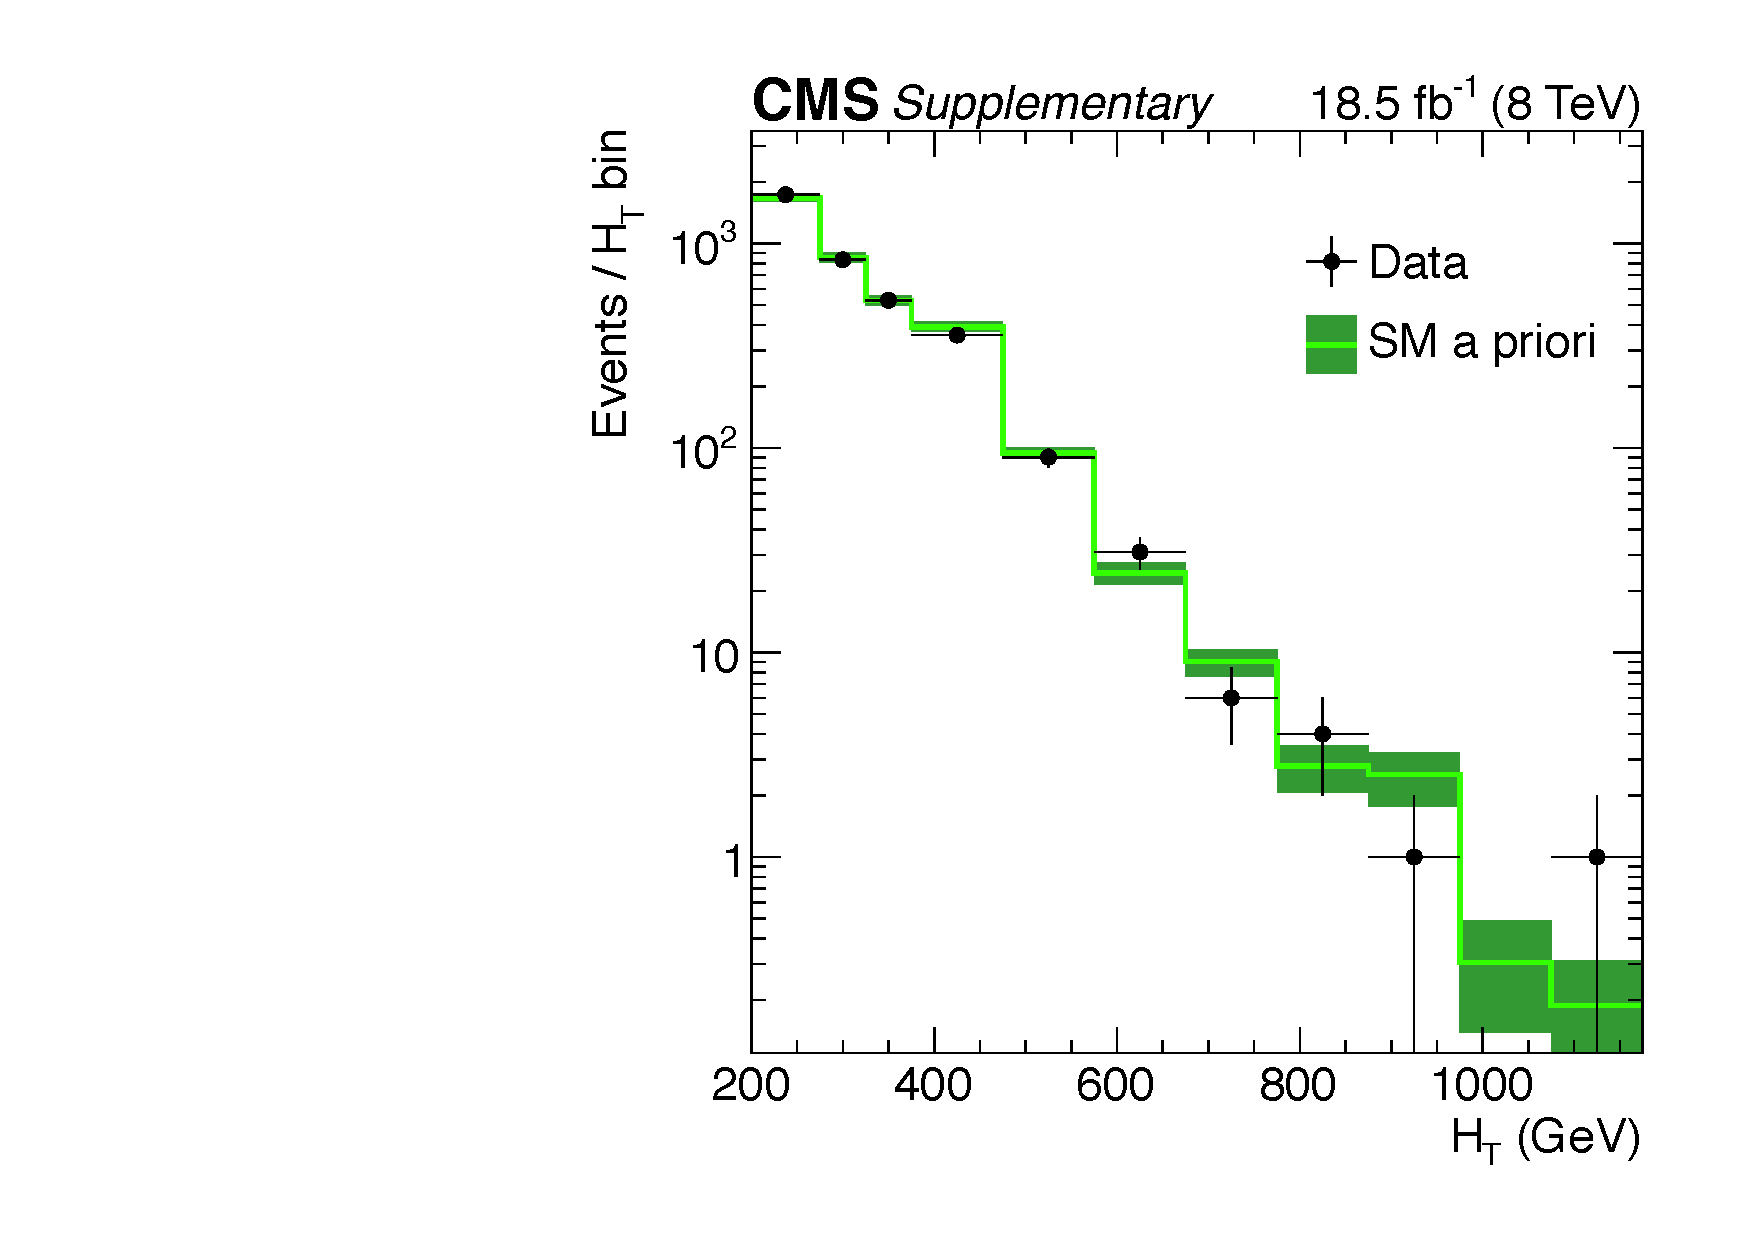
\includegraphics[width=0.7\textwidth]{RootFilesAndTarFiles/eq1b_le3j_prefit_log} 
    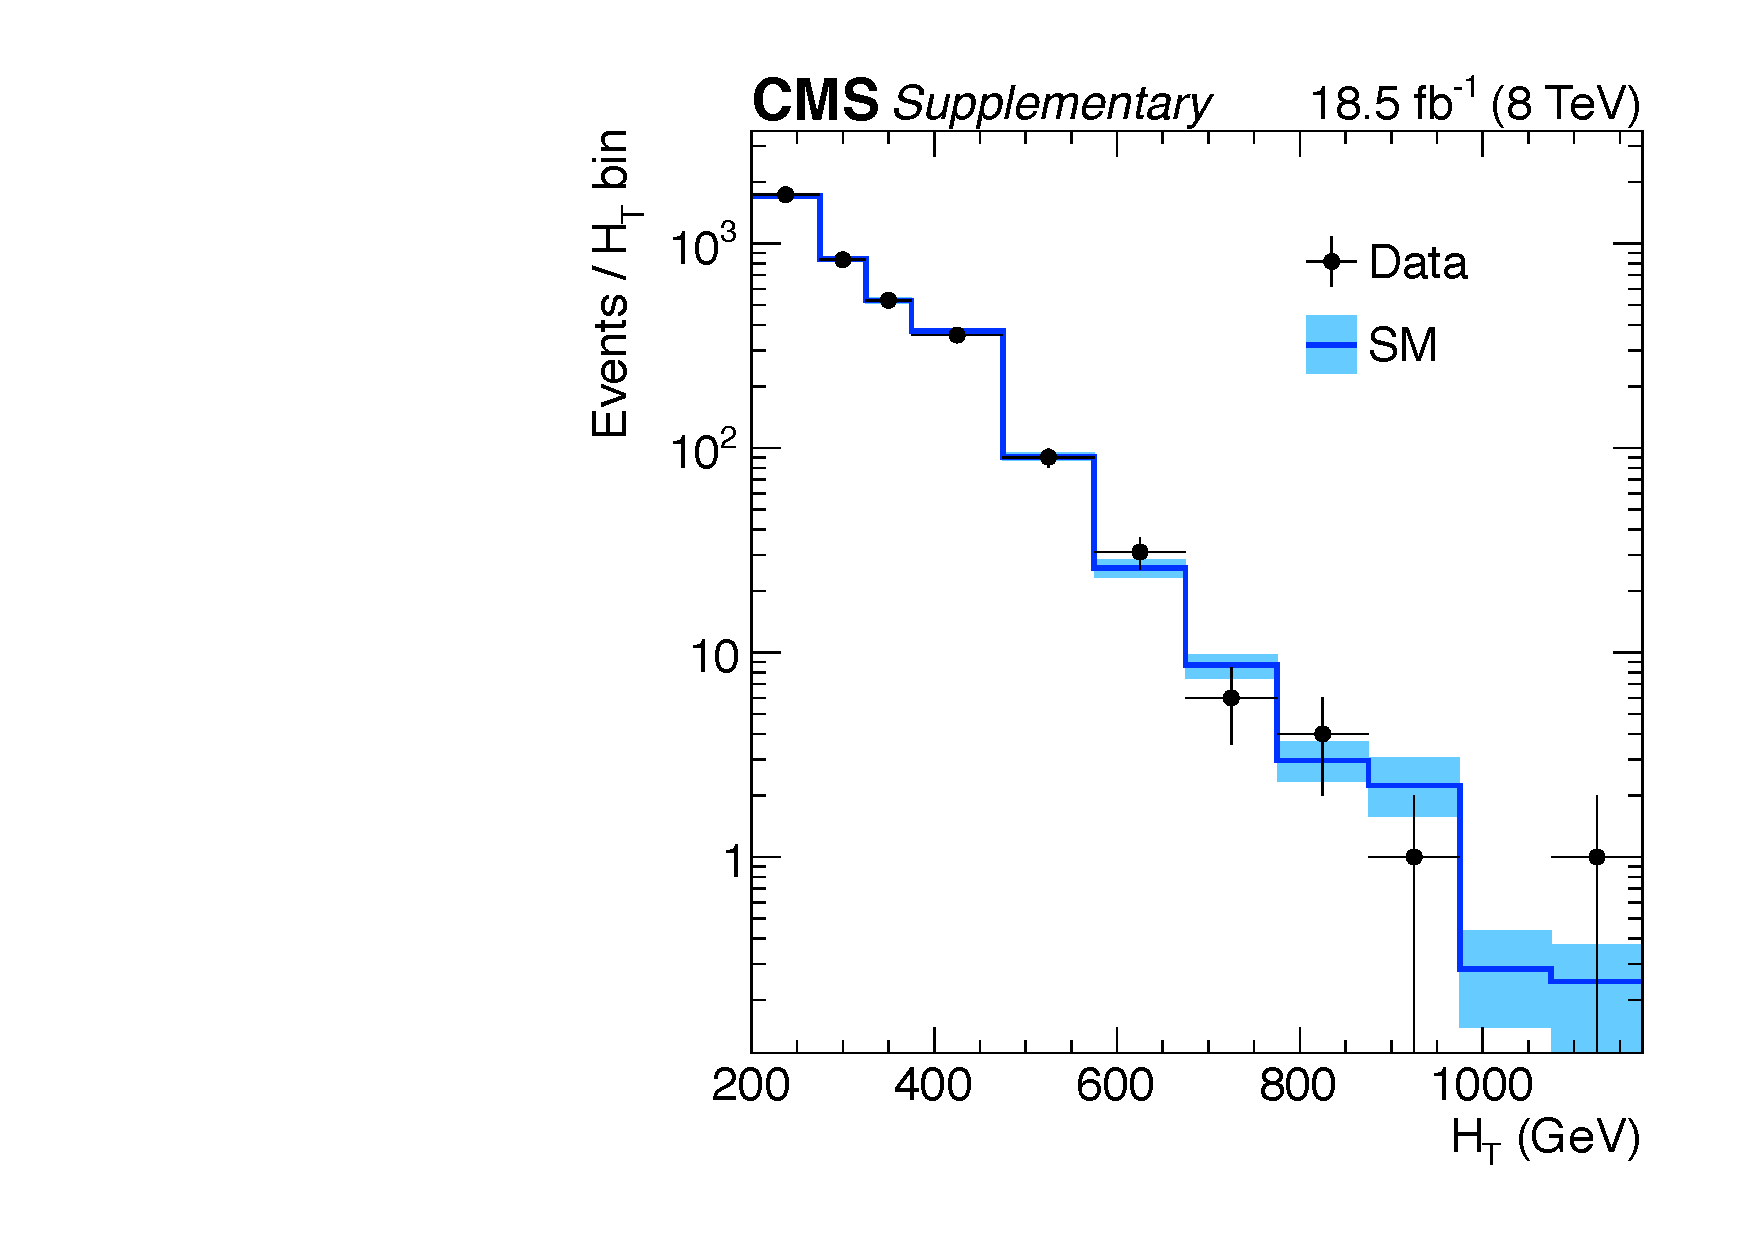
\includegraphics[width=0.7\textwidth]{RootFilesAndTarFiles/eq1b_le3j_postfit_log} \\
    \caption{\label{fig:best-fit-0b} Candidate signal event yields
      observed in data (solid circles) and SM expectations with their
      associated uncertainties (solid lines with bands) in bins of
      $H_\text{T}$ for events that satisfy $2 \geq n_\text{jet} \geq
      3$ and $n_\text{b} = 1$. (a) SM a priori
      expectations. (b) SM expectations from the fit including the
      signal region. }
  \end{center}
\end{figure}

\clearpage
\begin{figure}[h!]
  \begin{center}
    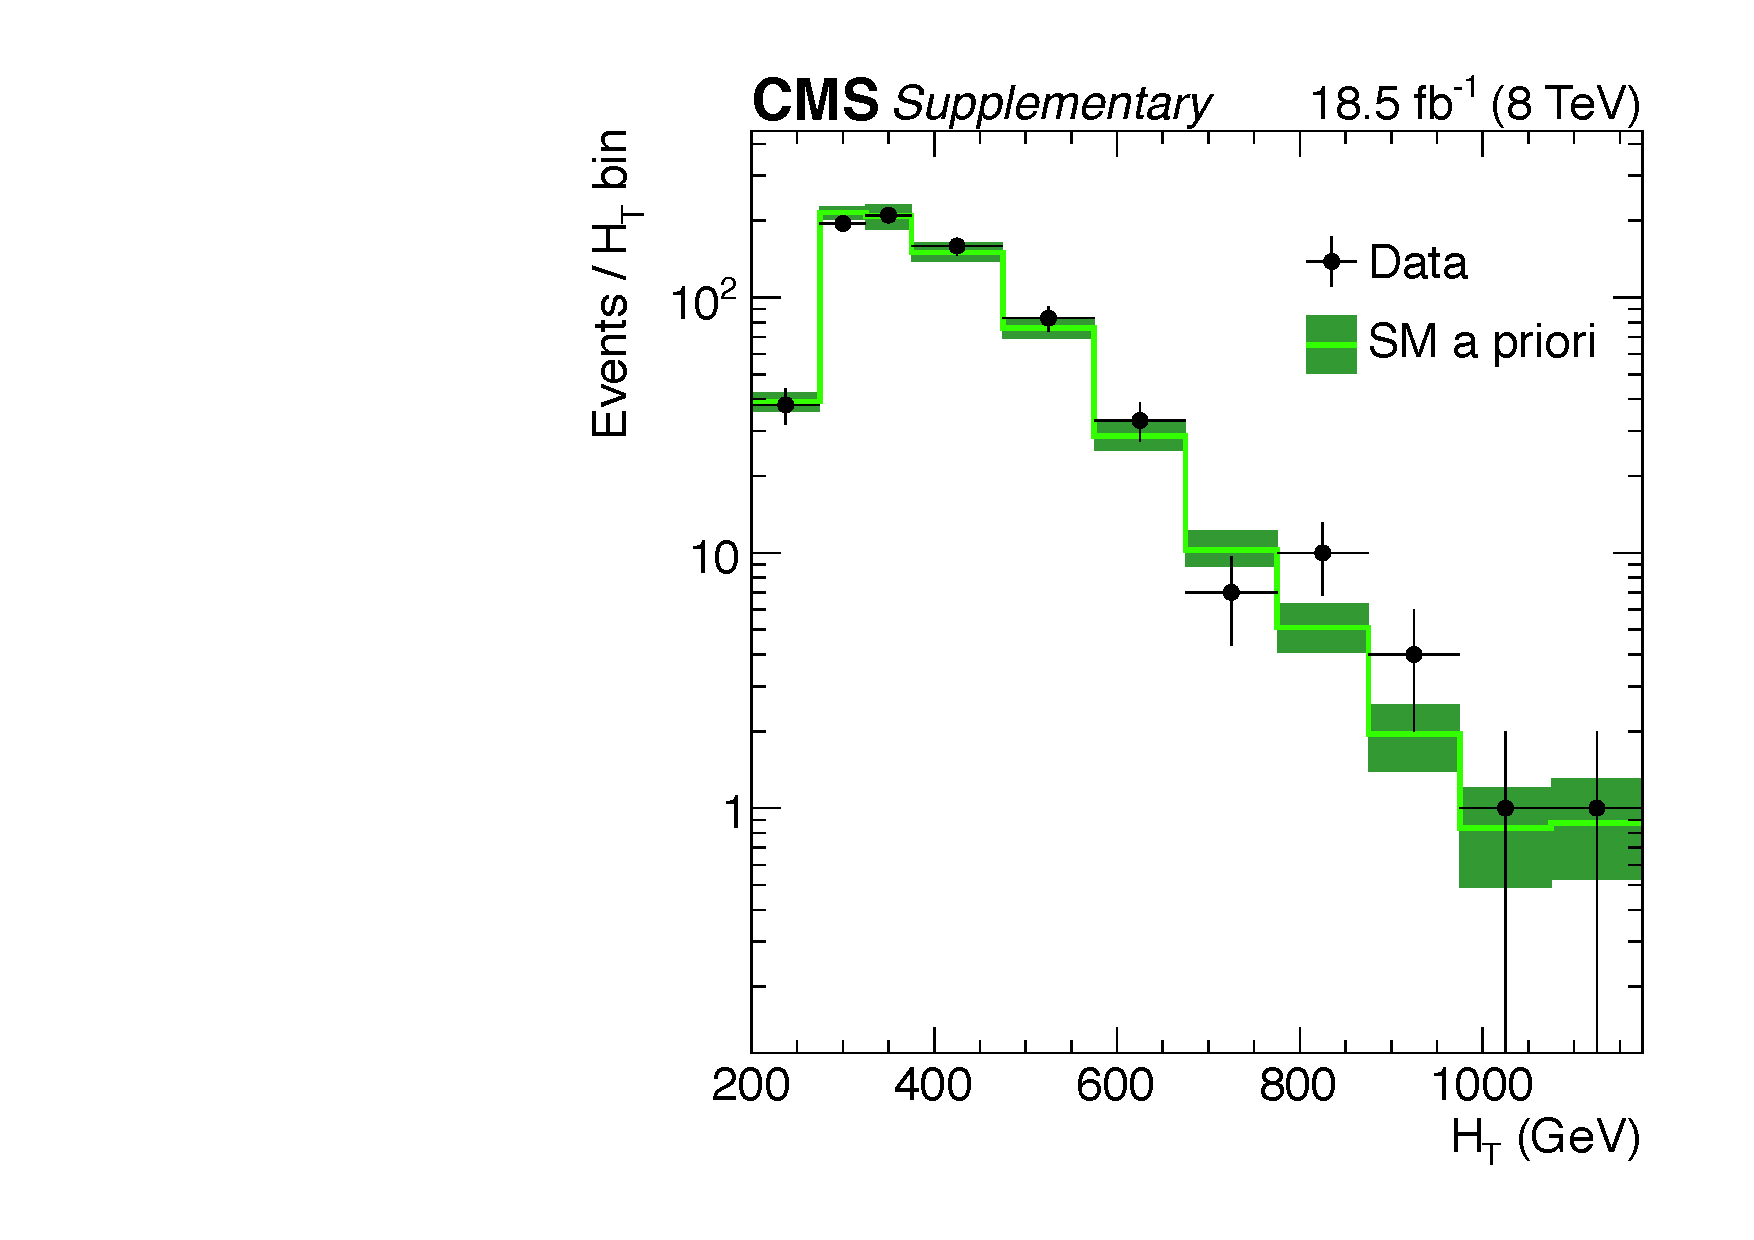
\includegraphics[width=0.7\textwidth]{RootFilesAndTarFiles/eq1b_ge4j_prefit_log} 
    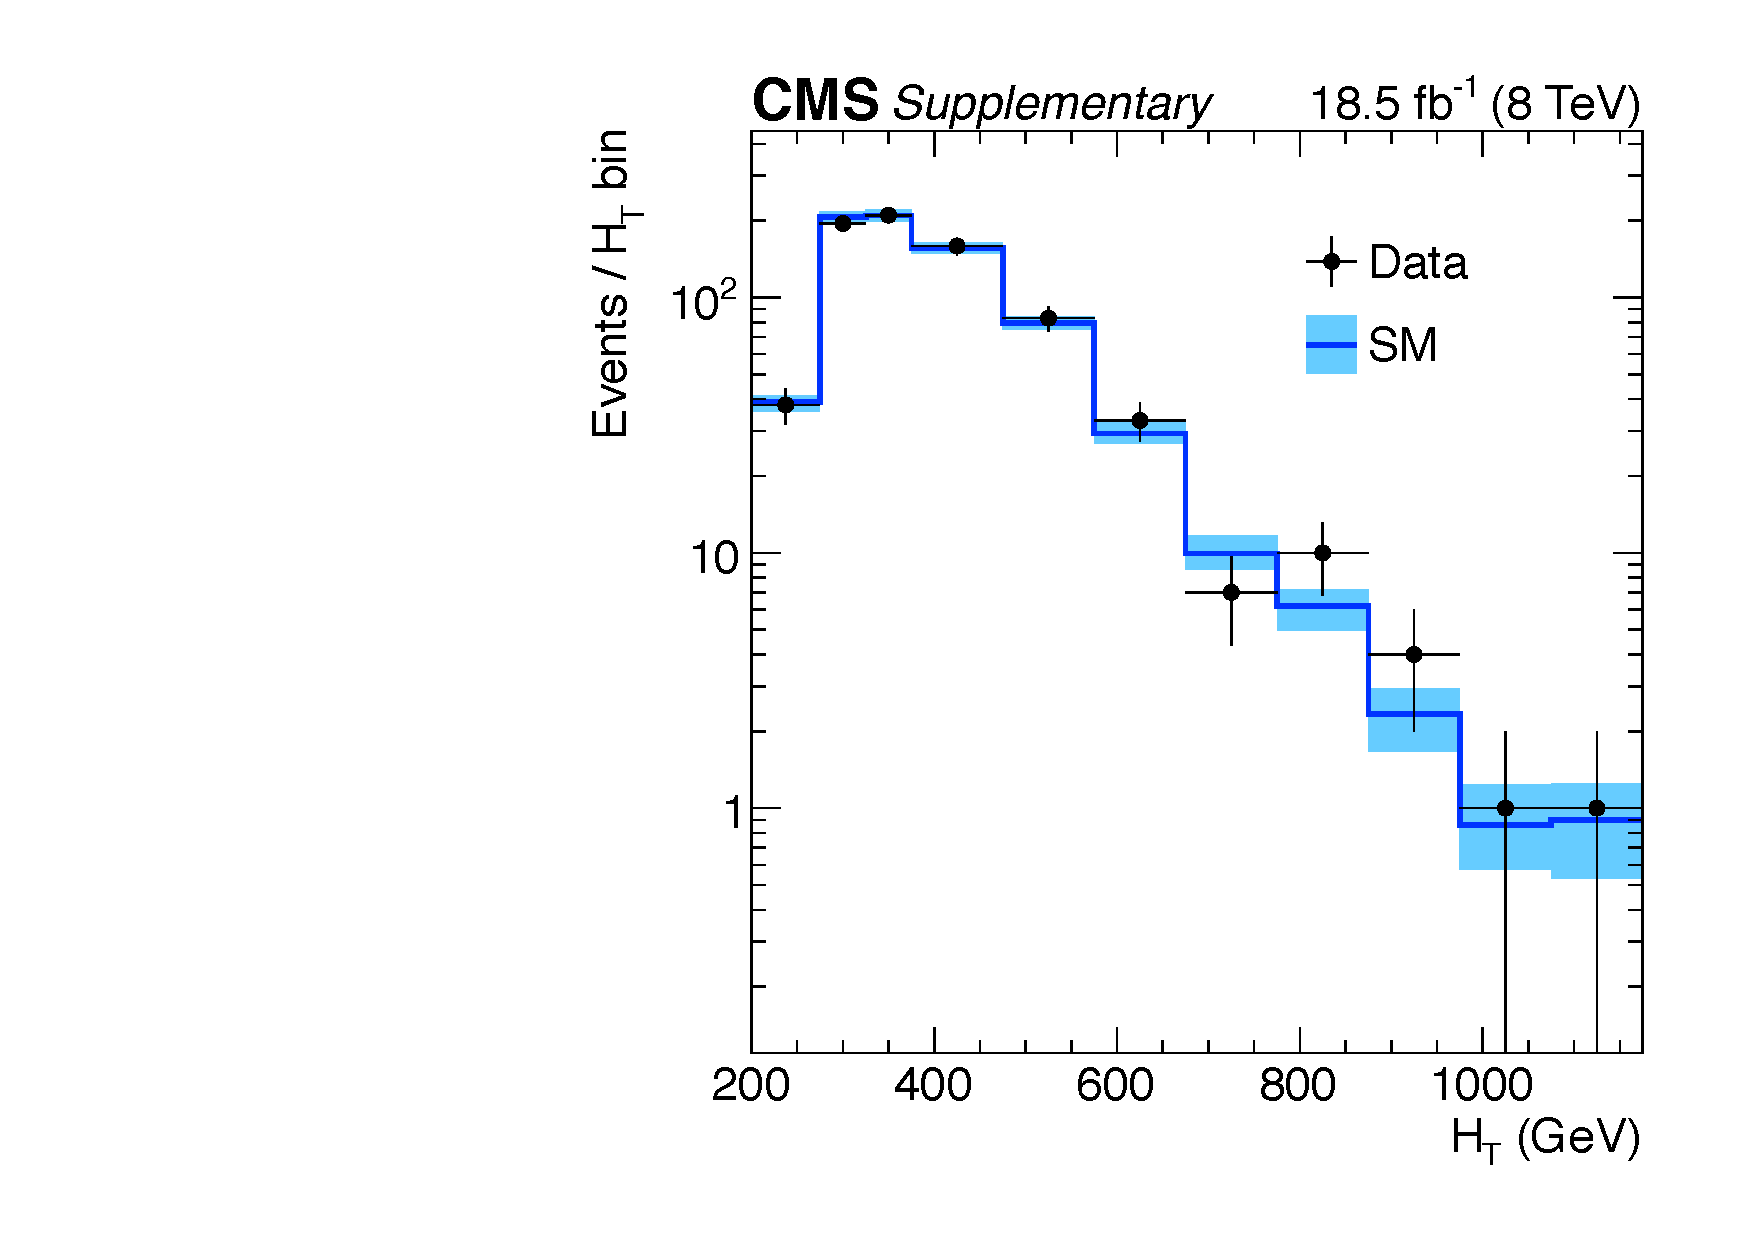
\includegraphics[width=0.7\textwidth]{RootFilesAndTarFiles/eq1b_ge4j_postfit_log} \\
    \caption{\label{fig:best-fit-0b} Candidate signal event yields
      observed in data (solid circles) and SM expectations with their
      associated uncertainties (solid lines with bands) in bins of
      $H_\text{T}$ for events that satisfy $n_\text{jet} \geq 4$ and
      $n_\text{b} = 1$. (a) SM a priori expectations. (b) SM
      expectations from the fit including the signal region. }
  \end{center}
\end{figure}

\clearpage
\begin{figure}[h!]
  \begin{center}
    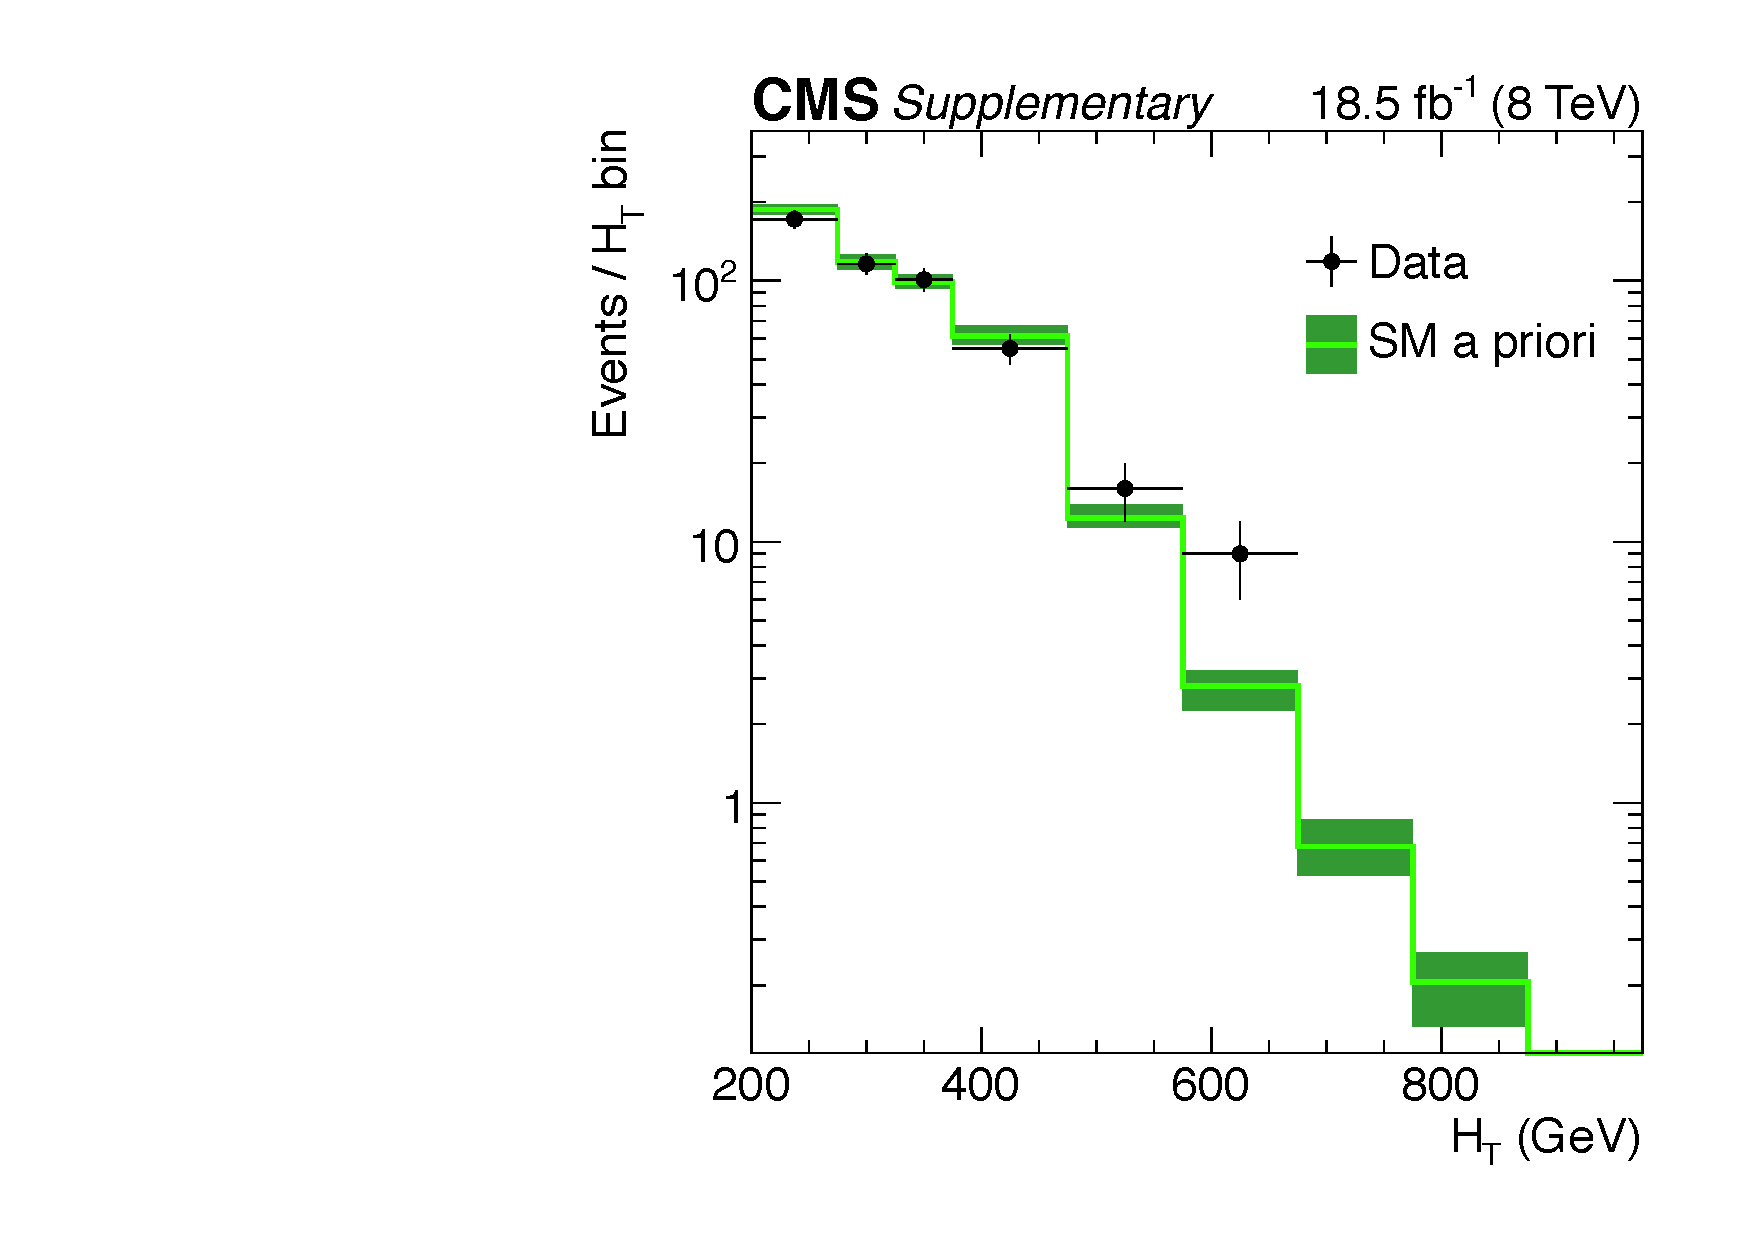
\includegraphics[width=0.7\textwidth]{RootFilesAndTarFiles/eq2b_le3j_prefit_log} 
    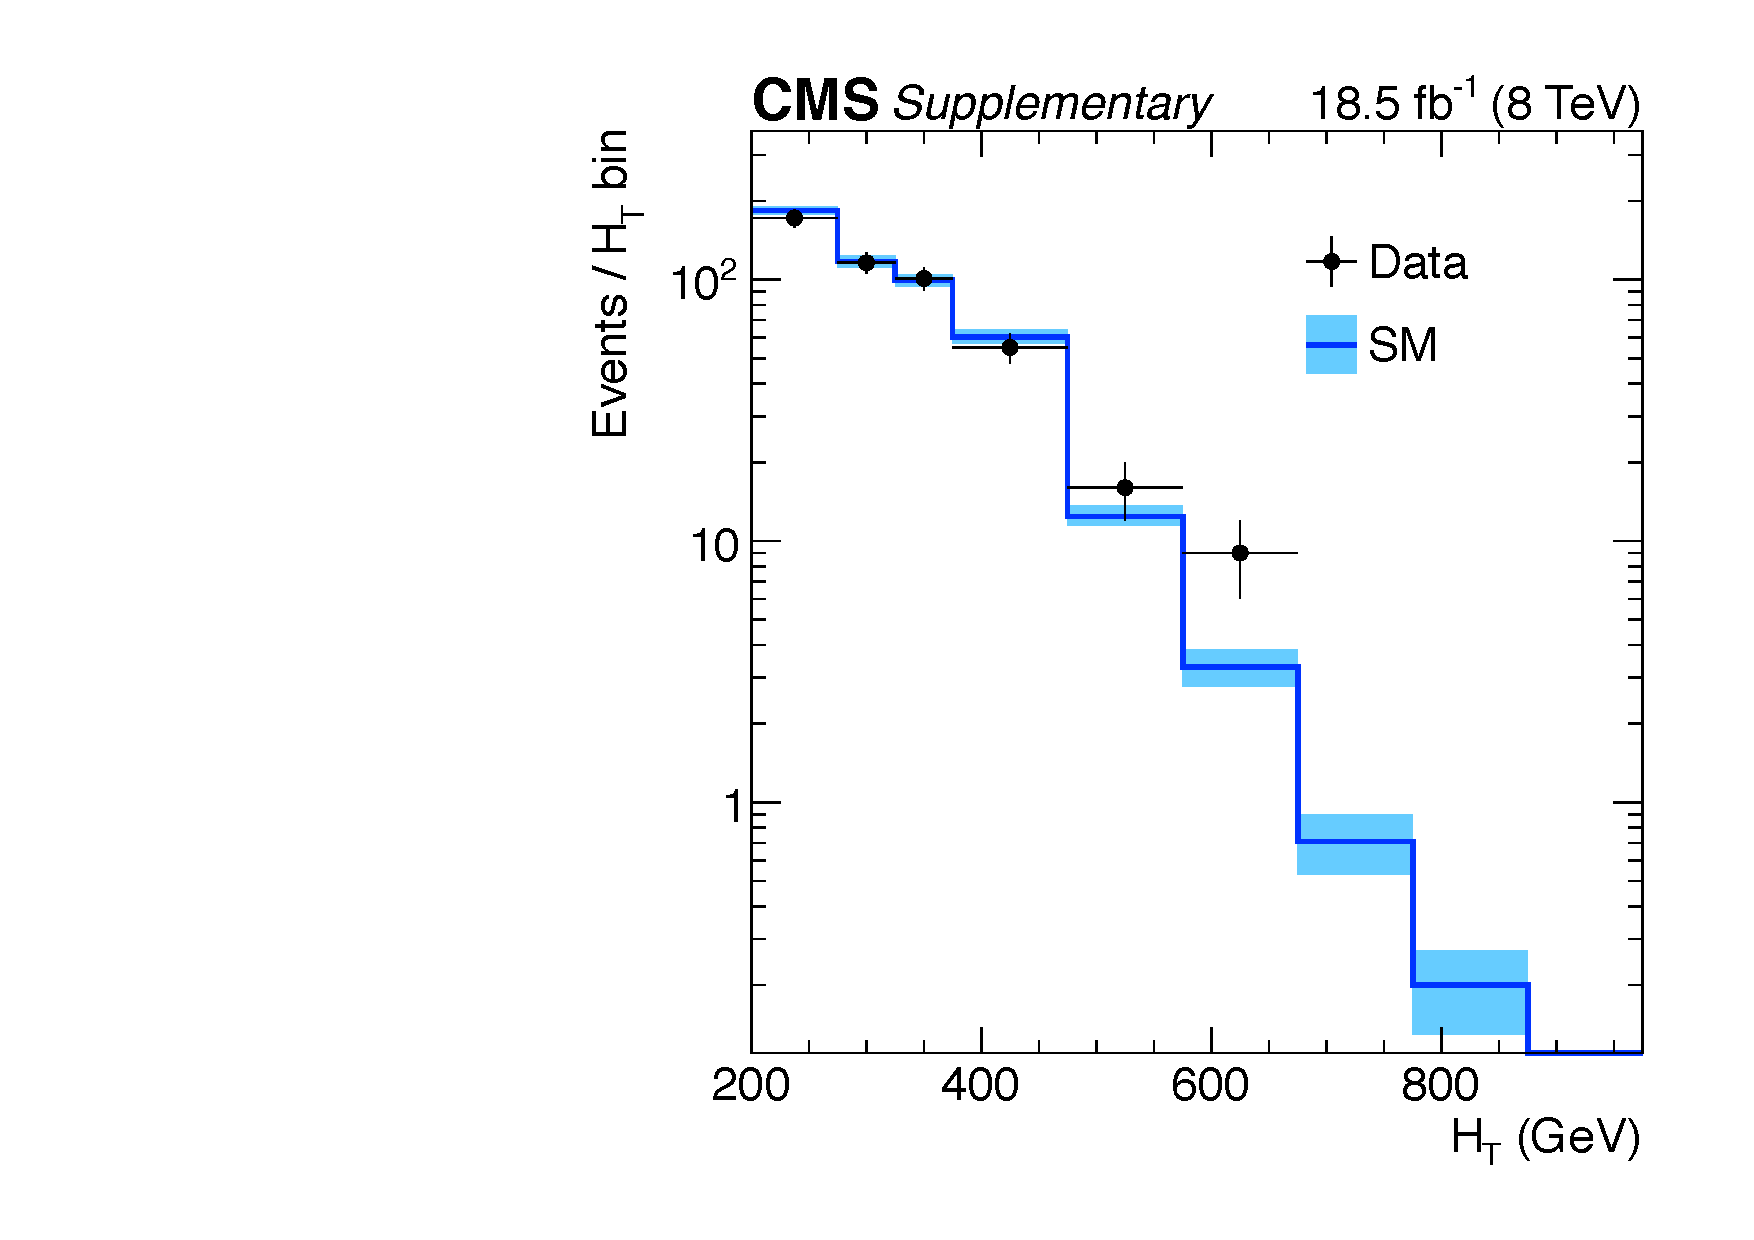
\includegraphics[width=0.7\textwidth]{RootFilesAndTarFiles/eq2b_le3j_postfit_log} \\
    \caption{\label{fig:best-fit-0b} Candidate signal event yields
      observed in data (solid circles) and SM expectations with their
      associated uncertainties (solid lines with bands) in bins of
      $H_\text{T}$ for events that satisfy $2 \geq n_\text{jet} \geq
      3$ and $n_\text{b} = 2$. (a) SM a priori
      expectations. (b) SM expectations from the fit including the
      signal region. }
  \end{center}
\end{figure}

\clearpage
\begin{figure}[h!]
  \begin{center}
    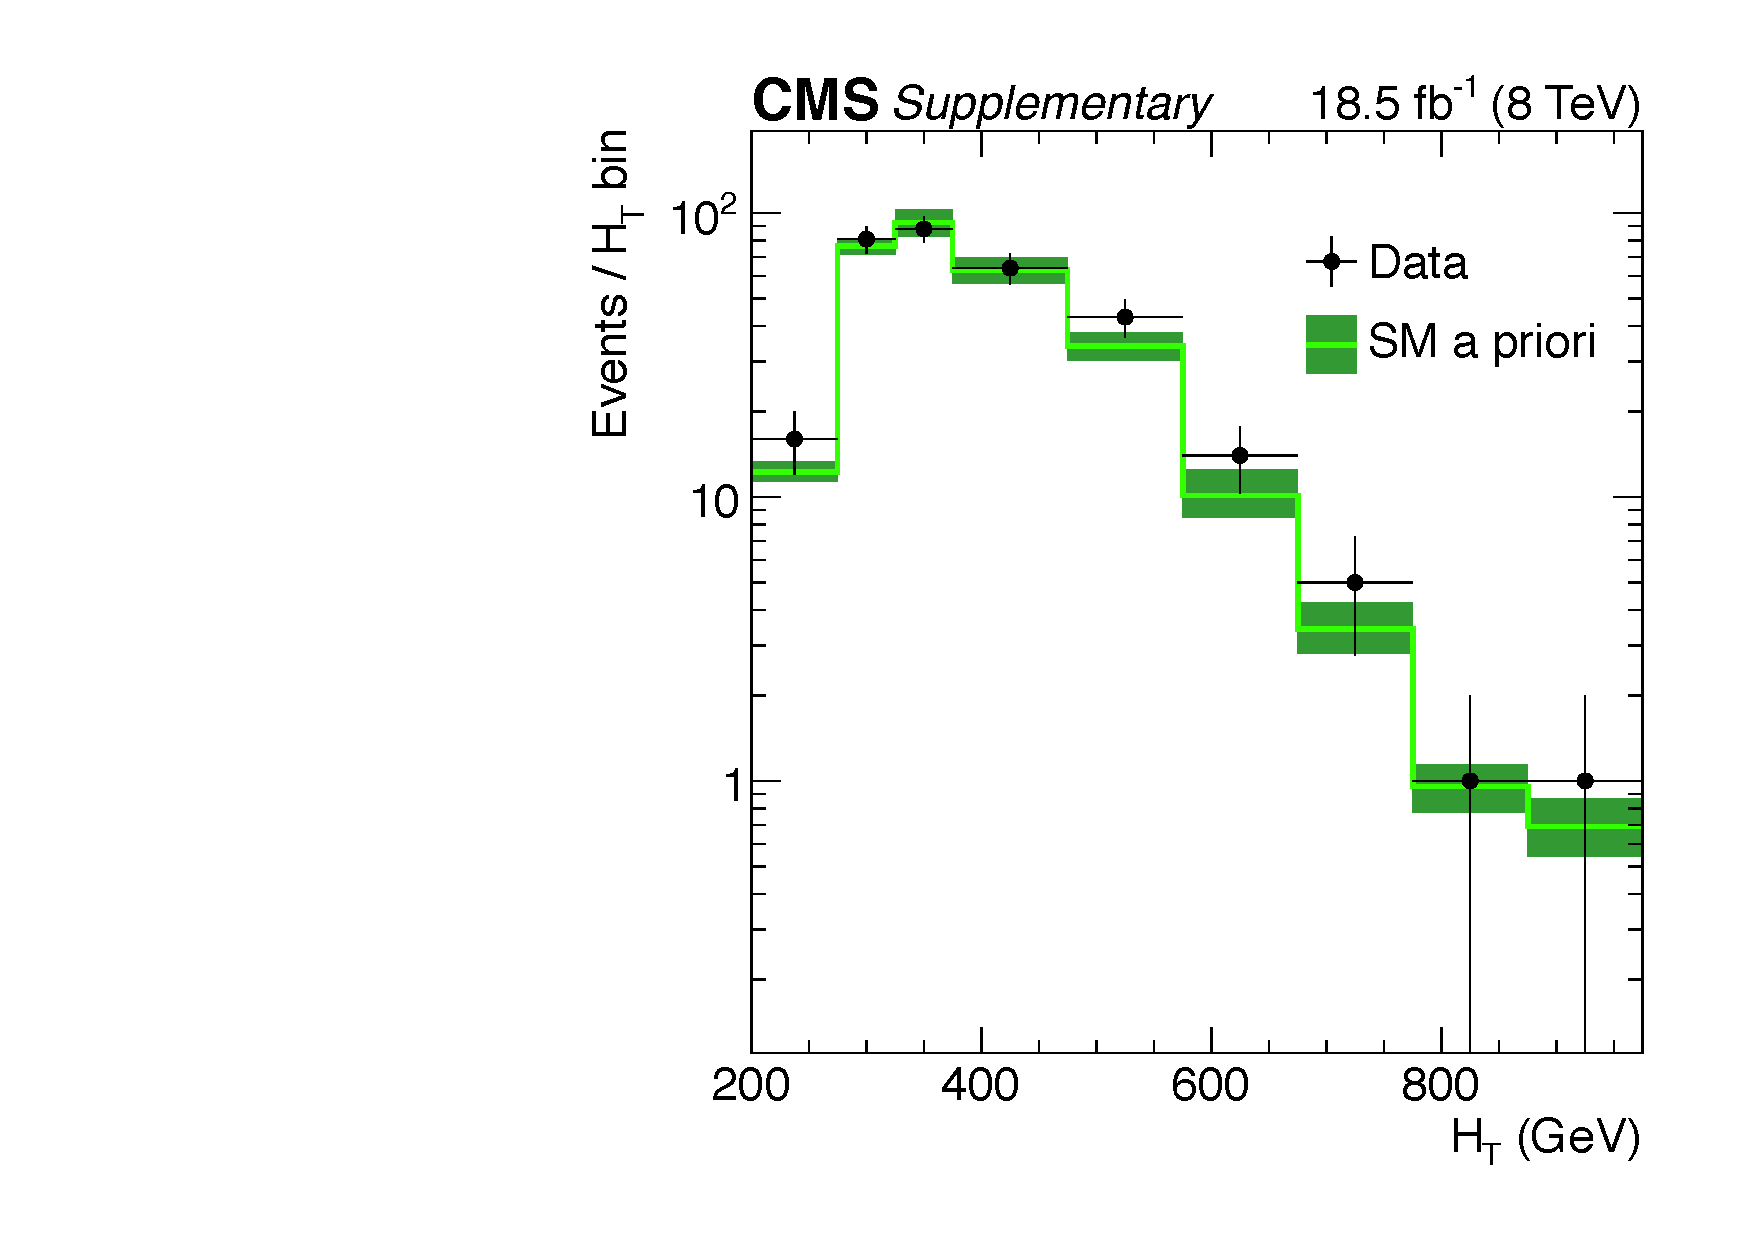
\includegraphics[width=0.7\textwidth]{RootFilesAndTarFiles/eq2b_ge4j_prefit_log} 
    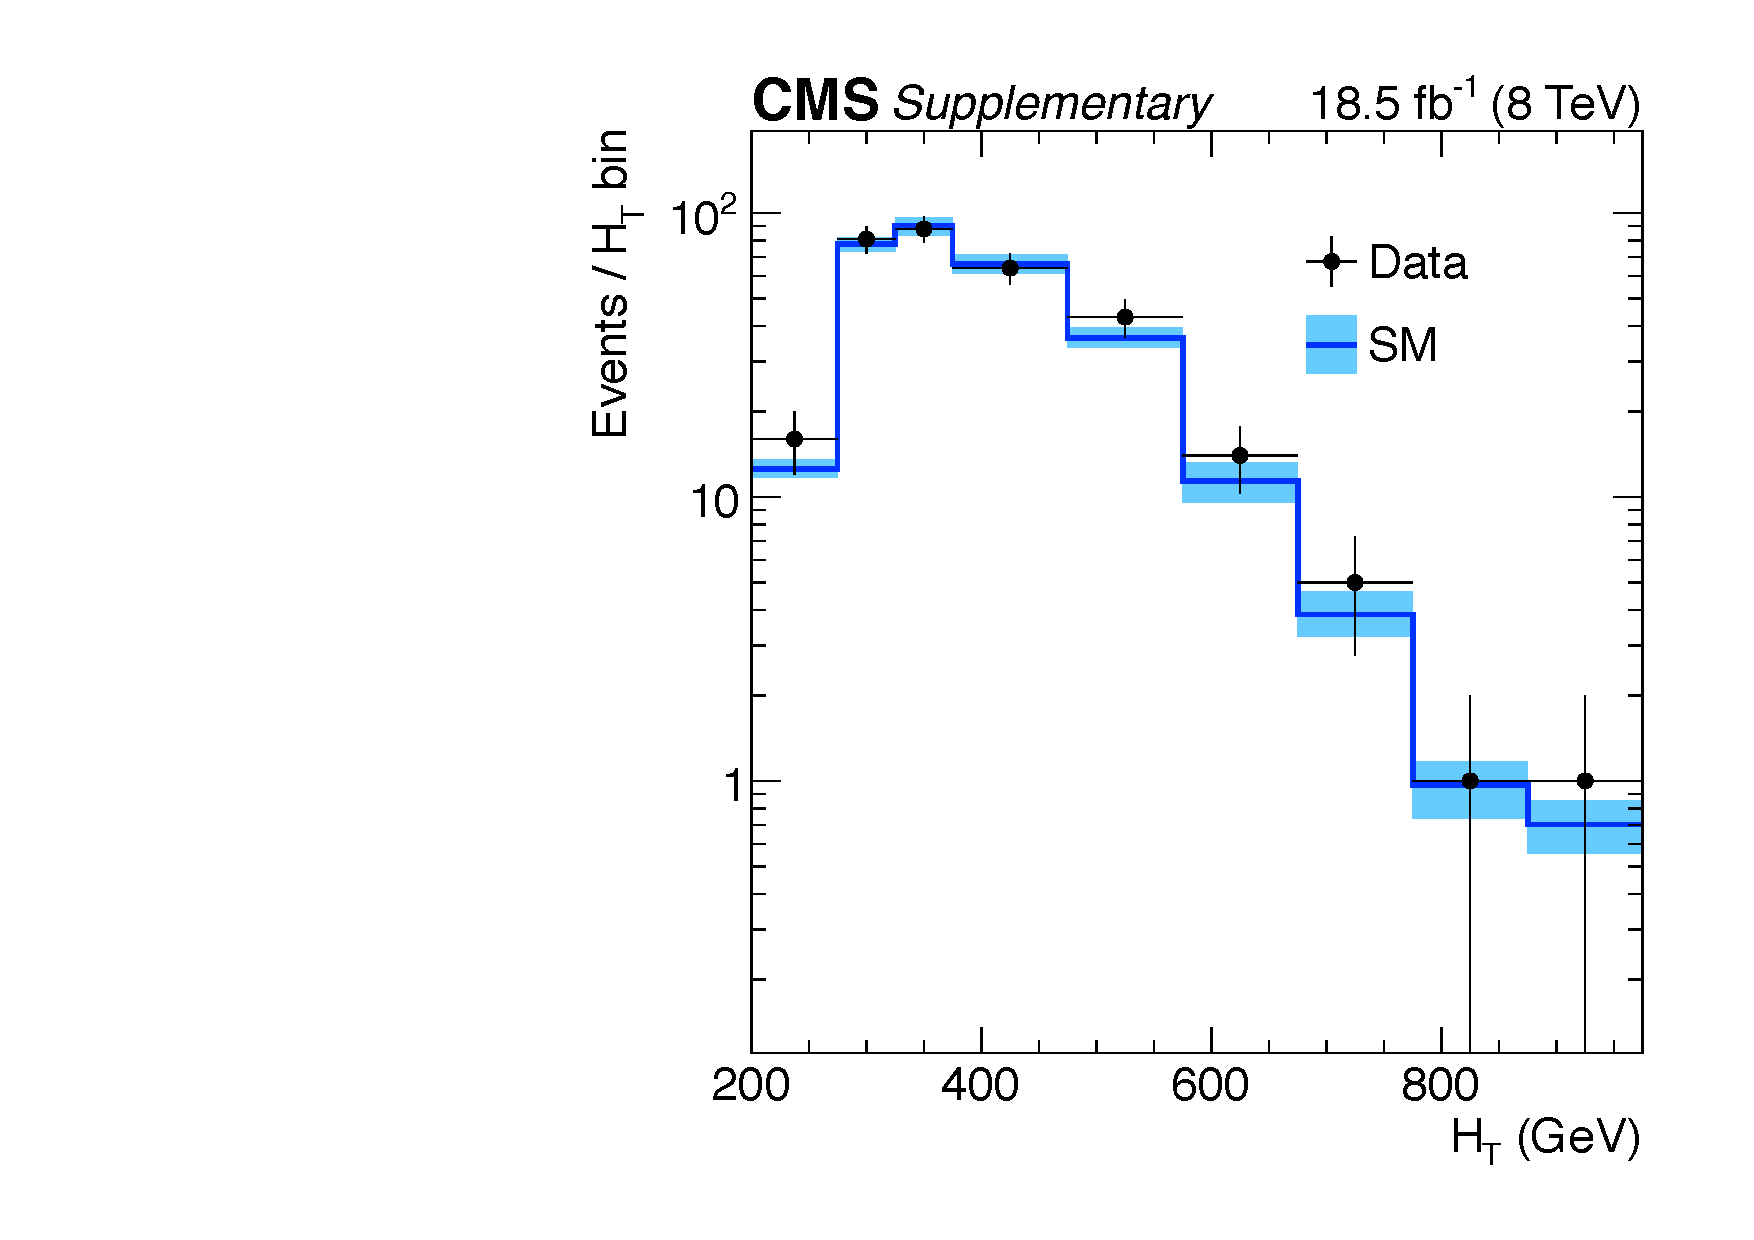
\includegraphics[width=0.7\textwidth]{RootFilesAndTarFiles/eq2b_ge4j_postfit_log} \\
    \caption{\label{fig:best-fit-0b} Candidate signal event yields
      observed in data (solid circles) and SM expectations with their
      associated uncertainties (solid lines with bands) in bins of
      $H_\text{T}$ for events that satisfy $n_\text{jet} \geq 4$ and
      $n_\text{b} = 2$. (a) SM a priori expectations. (b) SM
      expectations from the fit including the signal region. }
  \end{center}
\end{figure}

\clearpage
\begin{figure}[h!]
  \begin{center}
    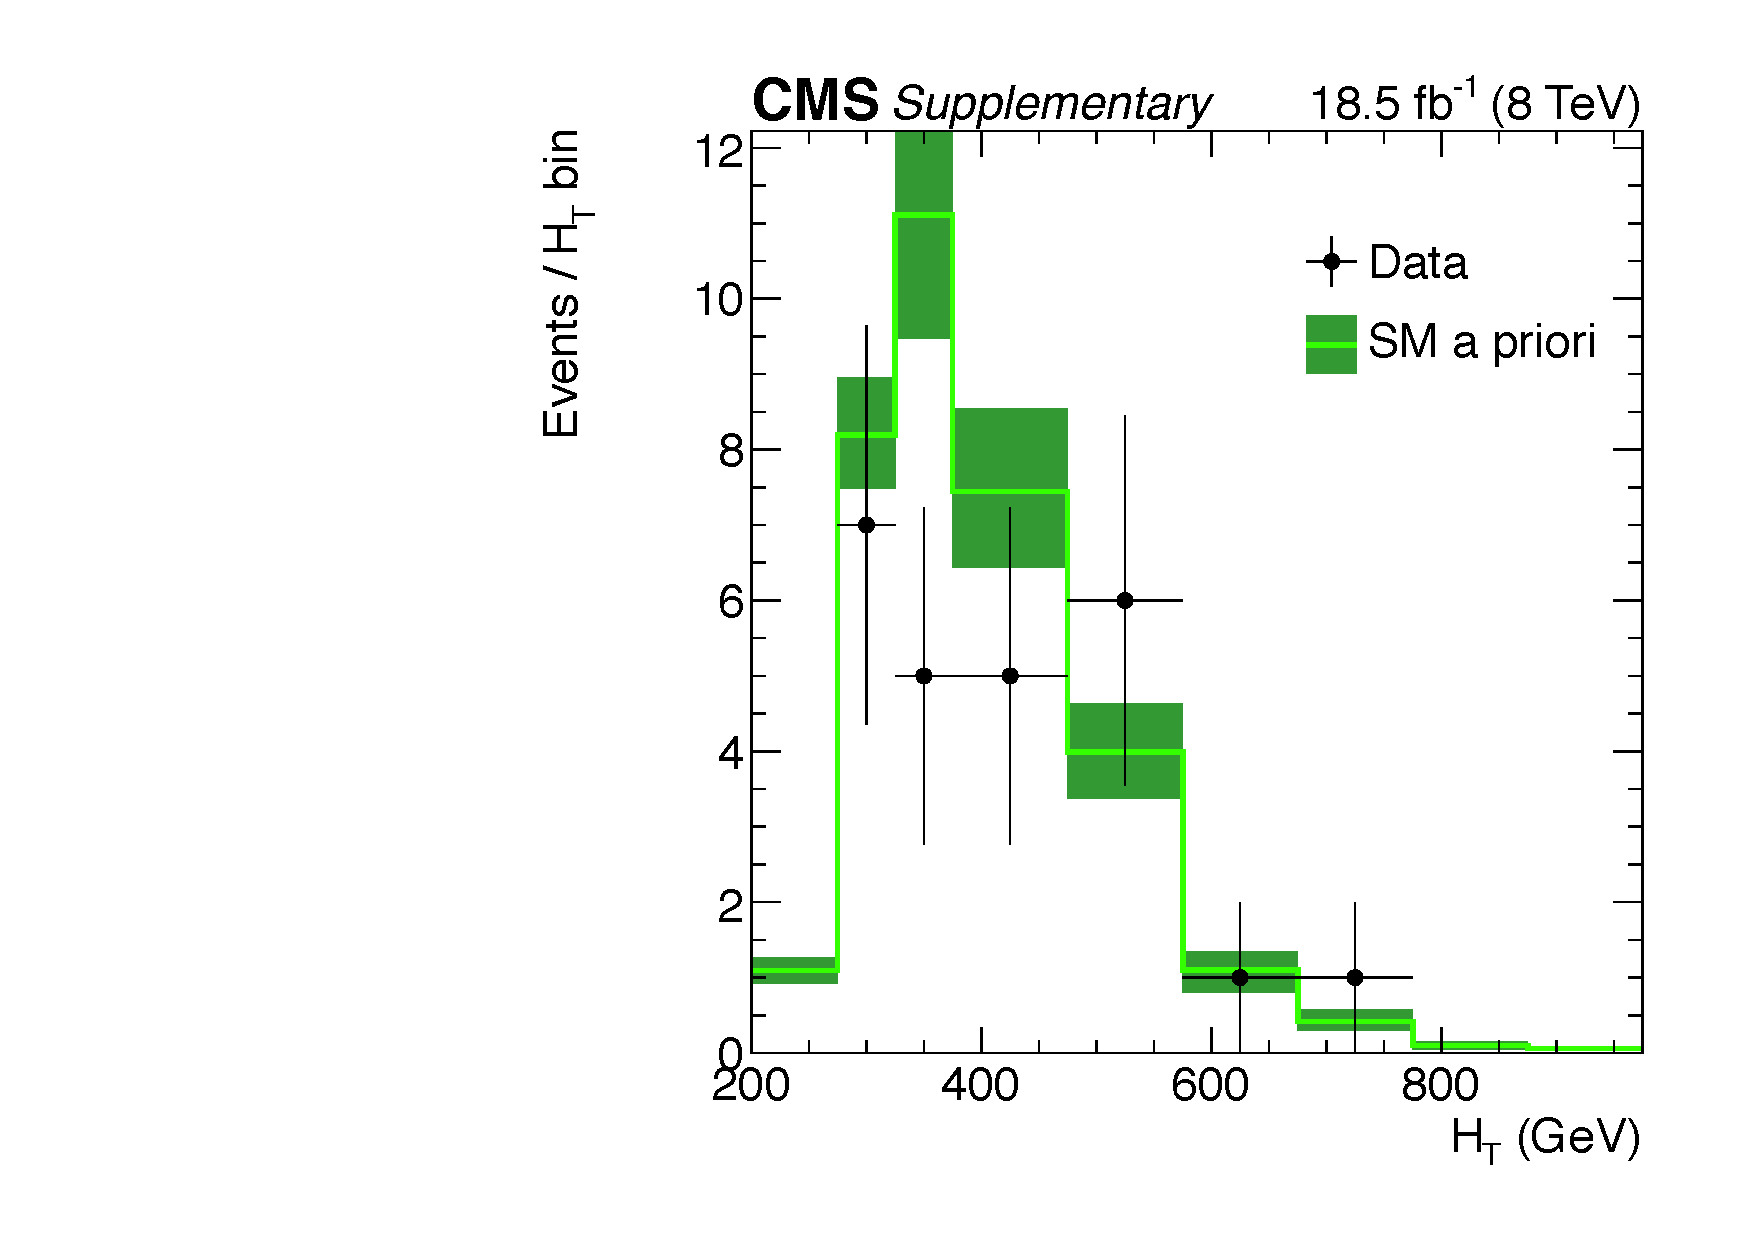
\includegraphics[width=0.7\textwidth]{RootFilesAndTarFiles/eq3b_ge4j_prefit_lin} 
    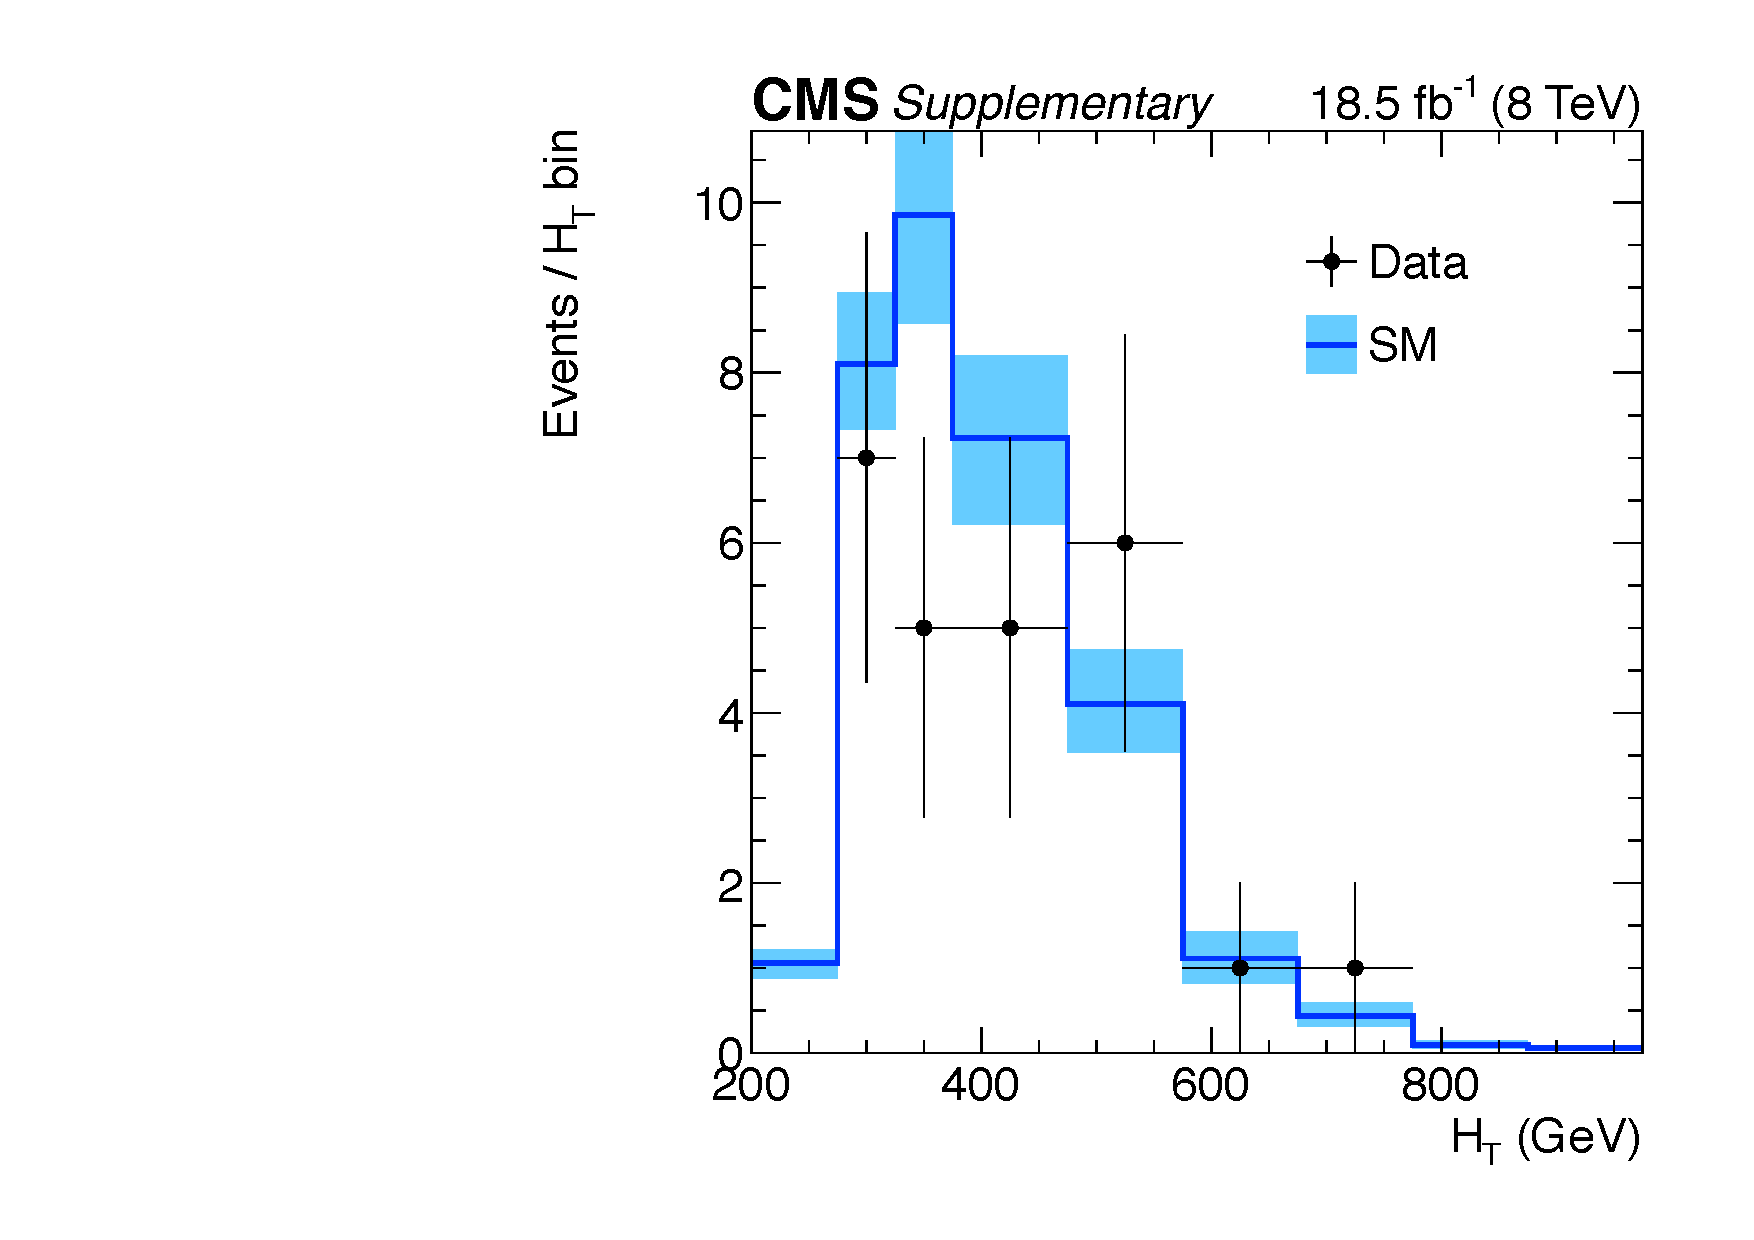
\includegraphics[width=0.7\textwidth]{RootFilesAndTarFiles/eq3b_ge4j_postfit_lin} \\
    \caption{\label{fig:best-fit-0b} Candidate signal event yields
      observed in data (solid circles) and SM expectations with their
      associated uncertainties (solid lines with bands) in bins of
      $H_\text{T}$ for events that satisfy $n_\text{jet} \geq 4$ and
      $n_\text{b} = 3$. (a) SM a priori expectations. (b) SM
      expectations from the fit including the signal region. }
  \end{center}
\end{figure}

\clearpage
\begin{figure}[h!]
  \begin{center}
    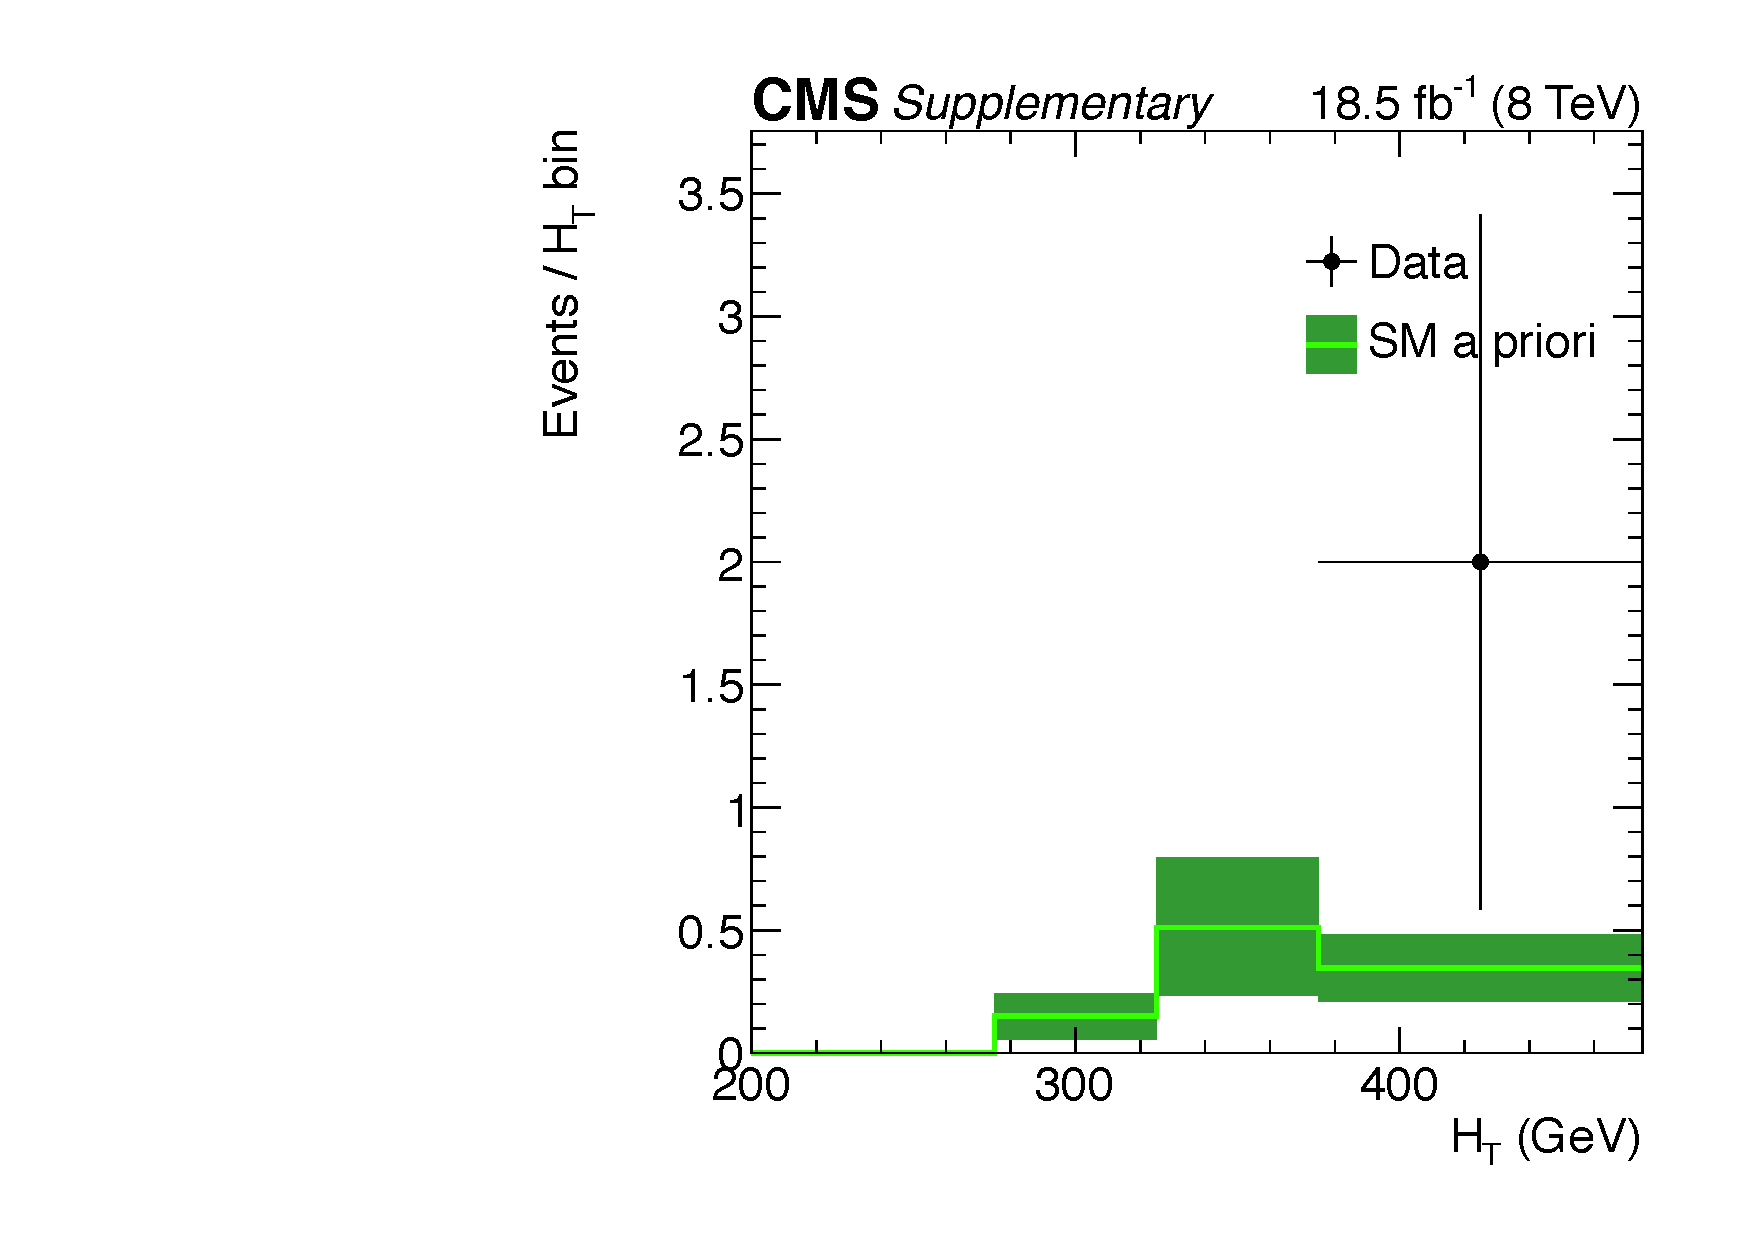
\includegraphics[width=0.7\textwidth]{RootFilesAndTarFiles/ge4b_ge4j_prefit_lin} 
    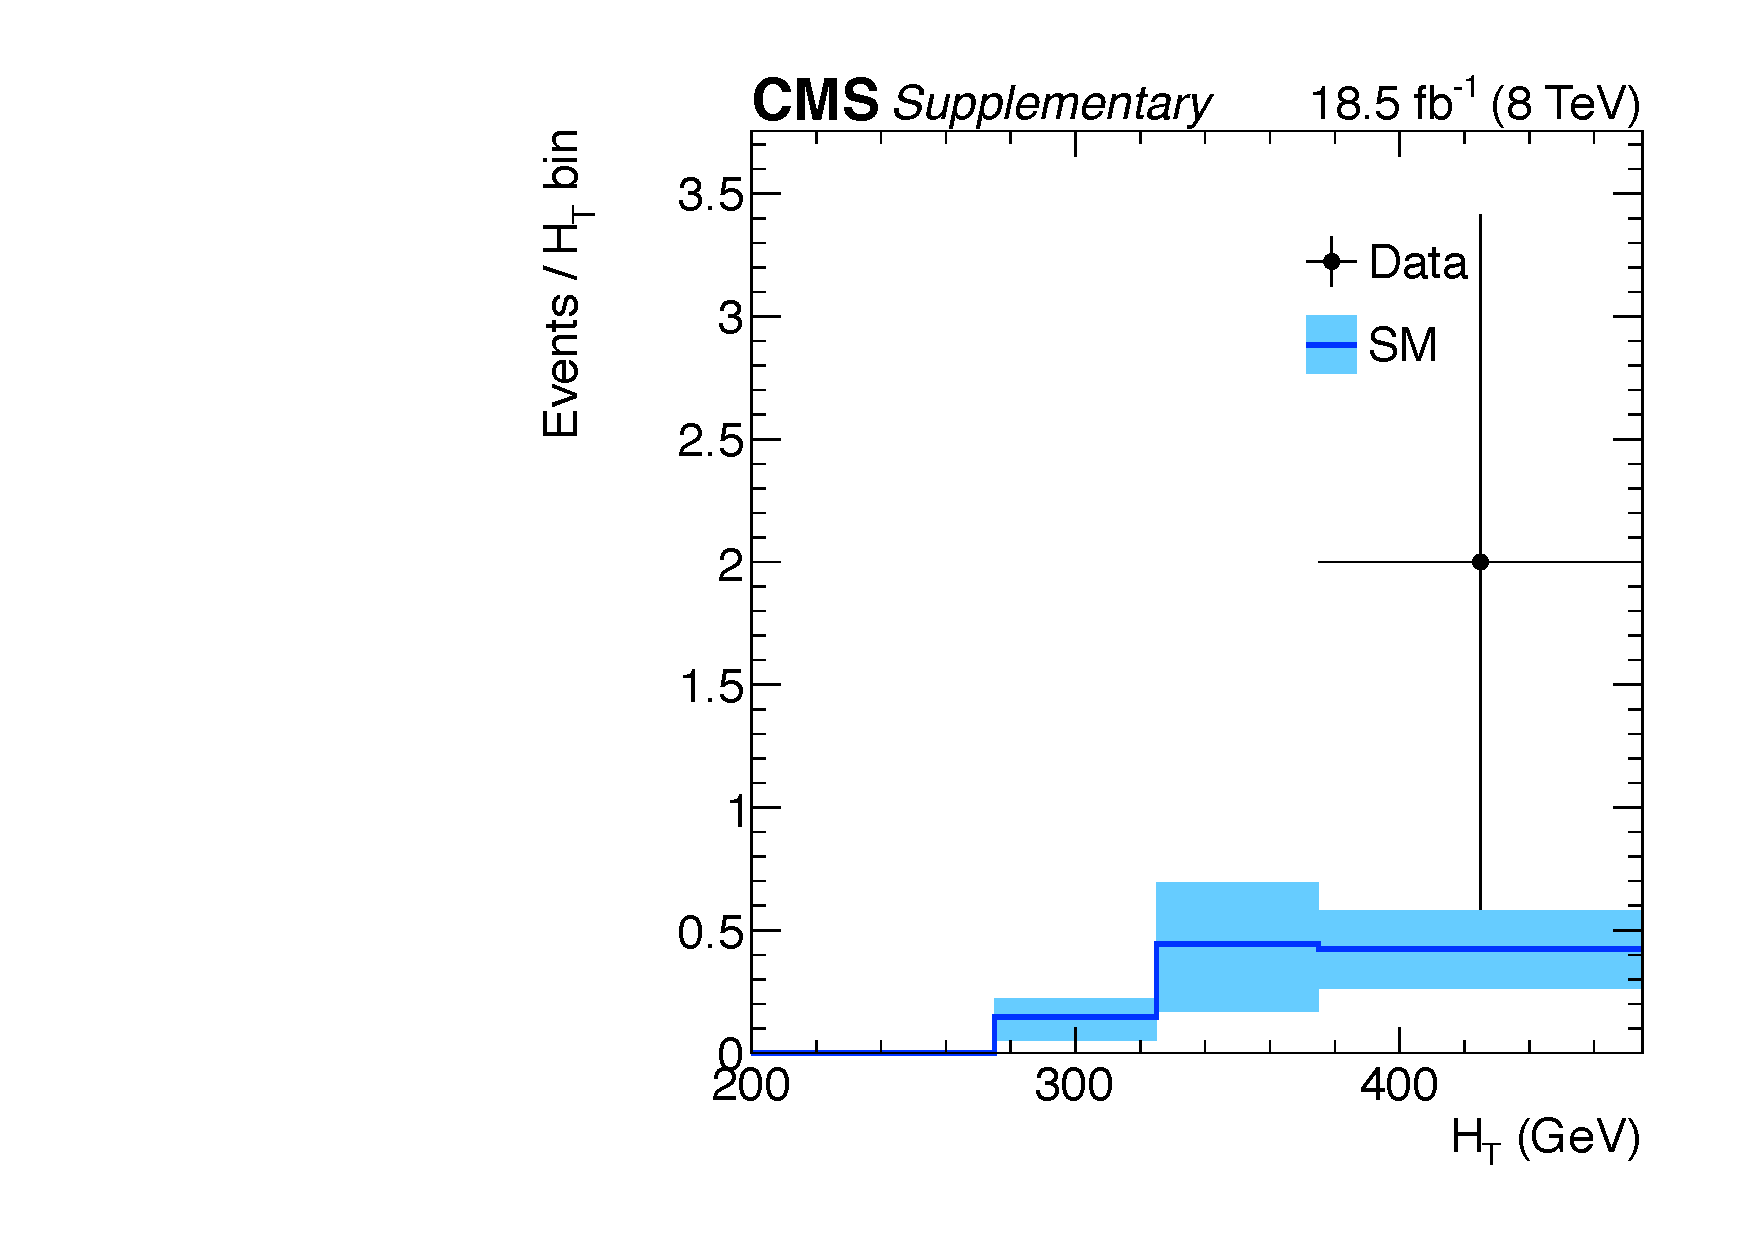
\includegraphics[width=0.7\textwidth]{RootFilesAndTarFiles/ge4b_ge4j_postfit_lin} \\
    \caption{\label{fig:best-fit-0b} Candidate signal event yields
      observed in data (solid circles) and SM expectations with their
      associated uncertainties (solid lines with bands) in bins of
      $H_\text{T}$ for events that satisfy $n_\text{jet} \geq 4$ and
      $n_\text{b} \geq 4$. (a) SM a priori expectations. (b) SM
      expectations from the fit including the signal region. }
  \end{center}
\end{figure}

%\bibliography{auto_generated}
